%%%%%%%%%%%%%%%%%%%%%%%%%%%%%%%%%%%%%%%%%%%%%%%%%%%%%%%
%% Bachelor's & Master's Thesis Template             %%
%% Copyleft by Artur M. Brodzki & Piotr Woźniak      %%
%% Faculty of Electronics and Information Technology %%
%% Warsaw University of Technology, 2019-2020        %%
%%%%%%%%%%%%%%%%%%%%%%%%%%%%%%%%%%%%%%%%%%%%%%%%%%%%%%%

\documentclass[
    left=2.5cm,         % Sadly, generic margin parameter
    right=2.5cm,        % doesnt't work, as it is
    top=2.5cm,          % superseded by more specific
    bottom=3cm,         % left...bottom parameters.
    bindingoffset=6mm,  % Optional binding offset.
    nohyphenation=false % You may turn off hyphenation, if don't like.
]{eiti/eiti-thesis}

\usepackage{gensymb}
\usepackage{tabularx}
\usepackage{makecell}
\usepackage{float}
\usepackage{ltablex}
\usepackage{xltabular}
\langpol % Dla języka angielskiego mamy \langeng
\graphicspath{{img/}}             % Katalog z obrazkami.
\addbibresource{bibliografia.bib} % Plik .bib z bibliografią

\begin{document}

%--------------------------------------
% Strona tytułowa
%--------------------------------------
\EngineerThesis % Dla pracy inżynierskiej mamy \EngineerThesis
\instytut{Telekomunikacji}
\kierunek{Telekomunikacja}
\specjalnosc{Teleinformatyka i Zarządzanie}
\title{
    Aplikacja do zarządzania warunkami \\
    technicznymi w pomieszczeniach biurowych \\
    oparta na architekturze mikrousługowej
}
\engtitle{ % Tytuł po angielsku do angielskiego streszczenia
    An application for managing \\
    internal conditions in office spaces \\
    based on microservices architecture
}
\author{\{Stanisław Skrzypek\}}
\album{300501}
\promotor{Dr hab. Inż. Prof. Artur Tomaszewski}
\date{\the\year}
\maketitle

%--------------------------------------
% Streszczenie po polsku
%--------------------------------------
\cleardoublepage % Zaczynamy od nieparzystej strony
\streszczenie 
Brak odpowiedniego zarządzania energią w budynkach biurowych od wielu lat 
powodował straty zarówno finansowe, jak i środowiskowe. Dodatkowo, w wyniku 
nieodpowiednich warunków panujących w pomieszczeniach pracy, osoby w nich 
przebywające nie mogły pracować w efektywny sposób. Celem tej pracy było 
zaproponowanie rozwiązania, za pomocą którego można byłoby mierzyć wartości 
kluczowych parametrów pomieszczeń biurowych, po czym podejmować stosowne 
działania mające na celu zarówno poprawienie komfortu pracowników, jak i 
redukcję zużywanej energii. Wykonano przegląd już istniejących prac naukowych 
dotyczących optymalnej wartości temperatury oraz natężenia światła w 
pomieszczeniach biurowych. Przygotowano system informatyczny oparty na 
architekturze mikrousługowej, który przyjmuje aktualne pomiary i je przetwarza. 
Przygotowano zestaw czujników, które wykonują pomiary oraz przesyłają 
je do systemu. 

%--------------------------------------
% Streszczenie po angielsku
%--------------------------------------
\newpage
\abstract
Lack of proper Energy management in office buildings has caused both 
financial, as well as environmental loss in many a year. Furthermore, as 
a result of inadequate room conditions, people staying in those rooms could 
not work effectively. The aim of this paper was to propose a solution by which 
it would be possible to measure the values of key parameters of office 
premises, and then take appropriate actions aimed at both improving the comfort 
of employees and reducing energy consumption. A review of the already existing 
scientific works on the optimal value of temperature and light intensity in 
offices was carried out. An IT system based on a microservice architecture was 
prepared, which takes current measurements and processes them. A set of sensors 
has been prepared that perform the measurements and send them to the system.

%--------------------------------------
% Oświadczenie o autorstwie
%--------------------------------------
\cleardoublepage  % Zaczynamy od nieparzystej strony
\pagestyle{plain}
\makeauthorship

%--------------------------------------
% Spis treści
%--------------------------------------
\cleardoublepage % Zaczynamy od nieparzystej strony
\tableofcontents

%--------------------------------------
% Rozdziały
%--------------------------------------
\cleardoublepage % Zaczynamy od nieparzystej strony
\pagestyle{headings}

\newpage % Rozdziały zaczynamy od nowej strony.
\section{Temat pracy}

Tematem niniejszej pracy jest utworzona w ramach seminarium dyplomowego aplikacja do 
zarządzania warunkami technicznymi w pomieszczeniach biurowych oparta na architekturze 
mikrousługowej. Produkt ma na celu poprawę warunków panujących w pomieszczeniach 
przeznaczonych do pracy codziennej. Wybrane parametry przeznaczone do optymalizacji to 
temperatura oraz natężenie światła.

Implementacja projektu przewiduje umieszczenie w badanych pomieszczeniach odpowiedniego 
rodzaju czujników, które będą na bieżąco monitorować stan danej przestrzeni. 
Zintegrowany z czujnikami system informacyjny powinien odczytywać przesyłane 
pomiary, a następnie je interpretować. Wynik interpretacji powinien być widoczny dla 
zainteresowanych osób. W wiadomości będą znajdować się informacje dotyczące 
akcji, które należy podjąć, aby umożliwić ustalenie się badanych parametrów na 
właściwym poziomie.

Utworzenie aplikacji miało przyczynić się do osiągnięcia dwóch głównych 
celów, stawianych od początku przygotowywania systemu:

\begin{enumerate}
    \item Poprawa warunków pracy - badania \cite{oseland2012} dowodzą, że 
    warunki panujące w pomieszczeniach do pracy mają wpływ na efektywność pracowników. 
    Utrzymanie ich na optymalnym poziomie może spowodować wzrost wydajności do 2,5\%
    \item Redukcja zużywanej energii - w praktyce często zdarza się, że po zakończeniu 
    pracy zostawiane są włączone światła na całą noc. Innym przykładem może być 
    sytuacja, w której pomieszczenie jest ogrzewane, mimo iż nikt z niego nie korzysta. 
    Przy wsparciu aplikacji będzie możliwe zapobieganie takim wydarzeniom, co w 
    konsekwencji ograniczy zużycie energii
\end{enumerate}

Zgodnie z wynikami badań opublikowanymi przez Institute for market transformation z 
2015 roku około 40\% całkowitej konsumpcji energii przypada na zasilanie budynków 
\cite{Imt.org2015}. Przekłada się to w ciągu roku na wydatek rzędu 450 miliardów 
dolarów. Najsłabiej zagospodarowane budowle zużywały od trzech do siedmiu razy więcej 
energii od tych najbardziej oszczędnych. Istnieje zatem potrzeba przygotowania 
i wdrożenia rozwiązań, które z jednej strony nie byłyby obciążające finansowo, z 
drugiej strony zaś ograniczające już istniejące koszty.          % Wygodnie jest trzymać każdy rozdział w osobnym pliku.
\newpage
\section{Istniejące rozwiązania}
Firma Sharp przygotowała podobne rozwiązanie, za pomocą którego można mierzyć kluczowe 
parametry danego pomieszczenia, przesyłać je na platformy chmurowe i je analizować 
\cite{sharp2022}. Różnica między tym produktem a rozwiązaniem proponowanym w tej pracy 
polega na tym, że w rozwiązaniu firmy Sharp czujniki są wbudowane w monitor służący 
jako centrum telekonferencyjne. W ten sposób wykonywane pomiary stają się niejako 
dodatkiem do monitora, niż głównym celem wstawienia urządzenia do konkretnej sali. 
W konsekwencji, wykonywanie pomiarów w wielu salach wiązałoby się z koniecznością 
zakupu drogiego monitora dla każdej z nich. Proponowane w tej pracy rozwiązanie zawiera 
jedynie zestaw czujników przesyłających pomiary do systemu, bez innych dodatków, co 
znacznie minimalizuje koszt wdrożenia takiego rozwiązania. Dzięki temu opłacalne staje
się zbieranie pomiarów z wielu sal jednocześnie.    % Umożliwia to również łatwą migrację do nowej wersji szablonu:
\newpage
\section{Założenia}
Treść sekcji zawiera zestawienie dwóch konkurencyjnych architektur wykorzystywanych do
projektowania systemów informatycznych: monolitycznej oraz opartej na mikrousługach.
Podrozdziały 4.1.1 - 4.1.4 przedstawiają zagadnienia, na które należy zwrócić
uwagę, przygotowując system utworzony z wielu modułów usługowych. W podrozdziale 4.1.5
spisano wszystkie moduły, które składają się na zaprojektowany w ramach niniejszej pracy 
system.

W tej sekcji przedstawiono główne założenia dotyczące rozwoju pracy, a także
przeprowadzono przegląd prac naukowych estymujących optymalną wartość temperatury
oraz natężęnia światła w pomieszczeniach biurowych.

Funkcjonalność i architektura systemu została zaprojektowana w oparciu o kilka istotnych 
założeń:

\begin{itemize}
    \item Szczególny nacisk jest położony na łatwość wdrożenia - system powinien być 
    gotowy do wdrożenia na środowisko 
    chmurowe. Organizacja zainteresowana uruchomieniem systemu dla swoich potrzeb 
    może wybrać opcję, w której dostarczane są obrazy odpowiednich mikroserwisów oraz 
    skrypty konfigurujące środowisko. Takie rozwiązanie mogłoby być ofertą skierowaną 
    do banków, które chcą zminimalizować ruch zewnętrzny. Może także skorzystać z 
    opcji, w której system jest hostowany na serwerach firmy będącej autorem 
    oprogramowania
    \item System składa się z czujników zbierających pomiary, które następnie przesyłane 
    są do mikroserwisów, które je przetwarzają. Do pomiaru zalicza się aktualna 
    temperatura oraz natężenie światła
    \item System oparty jest na regułach określających oczekiwaną wartość powyższych 
    parametrów w danej chwili czasu. Po otrzymaniu każdego z pomiarów porównywane są 
    wartości oczekiwane z rzeczywistymi i na tej podstawie przygotowywany jest wynik. 
    Domyślnie istnieje reguła podstawowa, gdzie oczekiwana temperatura wynosi 24.5
    \degree C, natomiast oczekiwane natężenie światła wynosi 550 lx. 
    Więcej informacji odnośnie ustalonych wartości zawarto 
    w tabeli \ref{tab:optymalna-temperatura} oraz tabeli \ref{tab:optymalne-natezenie}.
    \item System przewiduje dwie role użytkowników: pracowników danej 
    organizacji, którzy mogą tworzyć własne reguły dla pomieszczeń do nich 
    przypisanych, oraz administratorów organizacji, którzy posiadają wszystkie 
    uprawnienia przypisane pracownikom, a ponadto możliwość zarządzania informacjami 
    dotyczącymi organizacji, budynków, pomieszczeń i czujników
    \item System jest rozwijany przy wykorzystaniu platformy .NET w wersji 5.0
\end{itemize}

Tabela \ref{tab:optymalna-temperatura} pokazuje porównanie wyników z różnych artykułów traktujących 
o optymalnej temperaturze w pomieszczeniach:

\begin{xltabular}{1\textwidth}
    { |c|c| }
    \caption{Porównanie wyników badań estymujących optymalną temperaturę} \label{tab:optymalna-temperatura} \\
     \hline
     Badanie & Optymalna temperatura \\ 
     \hline
     \cite{Lan2012} & 23.5\degree C - 25.5\degree C \\ 
     \hline
     \cite{dai2014} & 23.0\degree C - 26.5\degree C \\ 
     \hline
     \cite{hedge2005} & 24.0\degree C - 25.0\degree C \\ 
     \hline
\end{xltabular}

W oparciu o powyższe badania wyliczono optymalną temperaturę jako średnią z uzyskanych
rezultatów. Jej wartość wynosi 24.5\degree C.
Natomiast w tabeli \ref{tab:optymalne-natezenie} porównywane są rezultaty badań nad optymalnym 
poziomem natężenia światła, który skutkował najlepszą efektywnością pracowników:

\begin{xltabular}{1\textwidth}
    { |c|c| }
    \caption{Porównanie wyników badań estymujących optymalne natężenie światła} \label{tab:optymalne-natezenie} \\
     \hline
     Badanie & Optymalne natężenie światła \\ 
     \hline
     \parencite{chinchiuan2014} & 500 lx \\ 
     \hline
     \parencite{liu2017} & 600 lx \\ 
     \hline
\end{xltabular}

W oparciu o powyższe badania wyliczono optymalne natężenie światła jako średnią z uzyskanych
rezultatów. Jej wartość wynosi 550 lx. % wystarczy podmienić swoje pliki main.tex i eiti-thesis.cls
                            % na nowe wersje, a cały tekst pracy pozostaje nienaruszony.
\clearpage
\section{Metodyka}

Największy nacisk w trakcie tworzenia pracy został położony na łatwość wdrożenia. 
W poniższych podrozdziałach przedstawiono kwestie, które należy wziąć pod uwagę
podczas projektowania rozwiązania, które ma tę cechę spełniać.

\subsection{Architektura systemu}

Wśród możliwych architektur systemów można wyłonić dwie najważniejsze gałęzie: 
architektura monolityczna lub oparta na mikrousługach, które są małymi, niezależnymi 
od siebie modułami, wspólnie ze sobą współpracującymi. Pierwsza z opcji opiera się 
na idei polegającej na tym, że wszystkie usługi oferowane przez dany system są zamknięte 
w jednym projekcie i funkcjonują jako całość. Druga możliwość opiera się na 
rozdzieleniu usług i umieszczeniu ich w oddzielnych modułach, które działają 
niezależnie od siebie. Obydwie architektury posiadają swoje wady i zalety i wybór 
jednej z nich zależy od specyficznych potrzeb każdego projektu. W tabeli 
\ref{tab:porownanie-architektur}. przedstawiono porównanie obydwu architektur 
\cite{newmanb2015}, które uwzględnia:

\begin{itemize} % lista nienumerowana
    \item Odporność systemu na awarie. Oferowane przez system usługi powinne być w każdym 
    momencie dostępne dla użytkowników
    \item Skalowalność. Potrzeba skalowania wynika ze zbyt dużego obciążenia dla jednego 
    lub większej liczby modułów w jednostce czasu. Brak dopasowania zasobów do 
    aktualnego zapotrzebowania może prowadzić do tego, że system nie będzie odpowiadał 
    na żądania użytkowników
    \item Łatwość wdrożenia. Architektura systemu nie powinna utrudniać wdrożenia nowych 
    funkcjonalności
    \item Zespół deweloperski. Architektura systemu nie powinna wymagać zatrudnienia 
    wielu programistów
\end{itemize}

    \begin{xltabular}{1\textwidth} { 
        | >{\arraybackslash}c 
        | >{\arraybackslash}X 
        | >{\arraybackslash}X | }
        \caption{Porównanie popularnych architektur systemów} \label{tab:porownanie-architektur} \\
        \hline
       Cecha & System monolityczny & System oparty na architekturze mikrousługowej \\
        \hline
       Odporność systemu na awarie & 
       W przypadku awarii w jednym punkcie, cały system przestaje działać & 
       Awaria jednego z modułów niekoniecznie musi oznaczać niesprawność całego systemu \\
       \hline
       Skalowalność & 
       Wymusza zwiększanie liczby uruchomionych instancji systemu, nawet w przypadku silnego 
       zapotrzebowania jedynie na część oferowanych usług & 
       Możliwość zwiększania liczby instancji tylko tych mikrousług, które w danym momencie są 
       silnie obciążone \\
      \hline
      Łatwość wdrożenia &
      Nawet mała zmiana w kodzie systemu monolitycznego wymaga ponownego wdrożenia całego 
      kodu &
      Możliwość szybkiego wdrożenia poprawek w obrębie danego mikroserwisu \\
      \hline
      Zespół deweloperski &
      Rozbudowany projekt zazwyczaj wymaga zespołu liczącego setki programistów, co 
      utrudnia komunikację i zmniejsza efektywność pracy &
      Nie wymaga rozbudowanego zespołu, możliwość oddelegowania małej grupy pracowników 
      do oddzielnych mikroserwisów \\
      \hline
    \end{xltabular}

Biorąc pod uwagę założenia dotyczące projektu, lepszą decyzją jest wykorzystanie architektury
mikrousługowej. Zestawienie z tabeli \ref{tab:porownanie-architektur} jasno wskazuje, że 
konsekwencją dokonanego wyboru jest szybsze wdrożenie kolejnych wersji systemu.

\subsubsection{Serwisy zorientowane usługowo}

Docelowo, system oparty na architekturze mikrousługowej powinien składać się z mikroserwisów 
zorientowanych usługowo (ang. \textit{service-oriented architecture}). Stanowią one 
konstrukcję, w której wiele modułów współpracuje ze sobą w celu zapewnienia zbioru 
funkcjonalności. Serwis oznacza tutaj oddzielny proces pracujący na danej maszynie. 
Procesy te komunikują się ze sobą przez sieć.

\subsubsection{Sprzężenie serwisów}

Architektura mikrousługowa opiera się na tym, że poszczególne mikroserwisy działają 
niezależnie od siebie. Dzięki temu zmiany wprowadzone w jednym z modułów nie powinny 
wymagać zmian w drugim. Ponadto wdrożenie danego mikroserwisu nie powinno wymagać 
jednoczesnego wdrożenia innych. O tak rozdzielonych mikroserwisach mówi się, że są ze sobą 
luźno sprzężone (ang. \textit{loose coupling}). Prawidłowo skonstruowany mikroserwis powinien 
wiedzieć jedynie tyle, w jaki sposób może komunikować się z innymi mikroserwisami w celu 
uzyskania wymaganych danych.

\subsubsection{Spójność mikroserwisów}
W prawidłowo skonstruowanym systemie mikrousługowym funkcjonalność związana ze 
sobą (np. w kontekście biznesowym) jest umieszczona w jednym miejscu. O tak 
zaprojektowanych modułach mówi się, że są one spójne (ang. \textit{high cohesion}). 
Przykładem 
błędnej implementacji może być edycja danych osobowych klienta w wielu mikroserwisach. 
Wtedy zmiana w jednym module może wymagać zmiany w innych.

\subsubsection{Wyznaczanie granic między mikroserwisami}

Jednym z wyzwań stojących przed projektantem systemu jest wyznaczenie granic między
mikroserwisami. Każdy z mikroserwisów powinien być niezależny od innych. Aby to osiągnąć, należy
skupić się na wyznaczeniu odrębnych modeli danych wykorzystywanych przez system
\cite{delatorre2015}.
Każdy z modeli może odgrywać różną rolę w kontekście biznesowym. Dzięki podziałowi
modelu danych na mniejsze fragmenty można utworzyć oddzielne moduły, każdy z których
będzie odpowiedzialny za osobny fragment. W konsekwencji uzyskiwana jest niezależność
mikroserwisów. Mogą one komunikować się między sobą w celu otrzymania wymaganych informacji.

\subsubsection{Architektura systemu do zarządzania energią w pomieszczeniach biurowych}

Opierając się na poprzednich podrozdziałach oraz w oparciu o założenia utworzono 
architekturę systemu będącego rezultatem tej pracy inżynierskiej. Rysunek 
\ref{fig:architektura-systemu} przedstawia pełny zestaw modułów składających się na 
całość rozwiązania:

\begin{figure}[h]
    \centering
    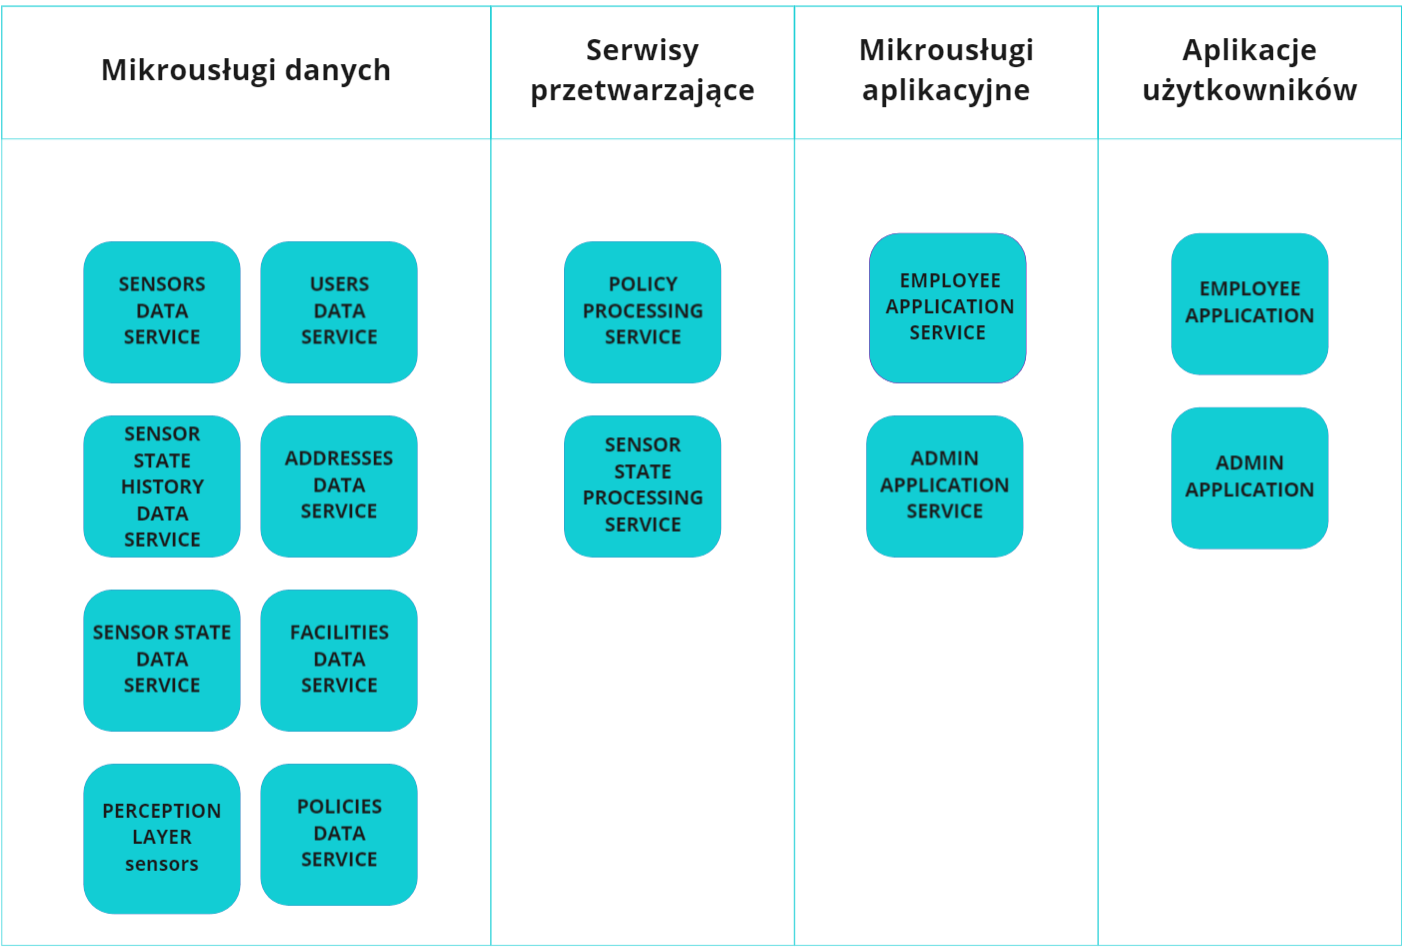
\includegraphics[width=1\textwidth]{architektura.jpg}
    \caption{Architektura systemu. Opracowanie własne}
    \label{fig:architektura-systemu}
\end{figure}

W tabeli \ref{tab:mikroserwisy-danych} opisano rolę mikroserwisów danych.

    \begin{xltabular}{1\textwidth} { 
        | >{\raggedright\arraybackslash}c        
        | >{\raggedright\arraybackslash}X | }
        \caption{Mikroserwisy danych} \label{tab:mikroserwisy-danych} \\
        \hline
       Nazwa & Funkcja \\
       \hline
       Addresses data service & 
       Przechowuje adresy organizacji oraz poszczególnych budynków \\
       \hline
       Facilities data service &
       Przechowuje szczegółowe dane dotyczące budynków \\
       \hline
       Policies data service & 
       Przechowuje reguły określające oczekiwaną wartość mierzonych parametrów \\
       \hline
       Sensors data service &
       Przechowuje szczegółowe dane dotyczące wykorzystywanych czujników \\
       \hline
       Sensor state history data service &
       Przechowuje historyczne pomiary z poszczególnych czujników \\
       \hline
       Sensor state data service &
       Przesyła pomiary od czujników \\
       \hline
    \end{xltabular}

Poza mikroserwisami danych aplikacja posiada również mikroserwisy przetwarzające 
dane, opisane w tabeli \ref{tab:serwisy-przetwarzajace}:

    \begin{xltabular}{1\textwidth} { 
        | >{\raggedright\arraybackslash}c        
        | >{\raggedright\arraybackslash}X | }
        \caption{Mikroserwisy przetwarzające} \label{tab:serwisy-przetwarzajace} \\
        \hline
       Nazwa & Funkcja \\
       \hline
       Sensor state processing service & 
       Otrzymuje dane z czujników. Zajmuje się ich prawidłowym zapisaniem, po czym wysyła 
       je dalej do PPS \\
       \hline
       Policy processing service &
       Przetwarza dane z czujników. Porównuje pomiary rzeczywiste z oczekiwanymi, które 
       zostały określone w regułach \\
       \hline
    \end{xltabular}

Na system składają się także mikroserwisy aplikacyjne opisane w tabeli \ref{tab:mikroserwisy-aplikacyjne}:

    \begin{xltabular}{1\textwidth} { 
        | >{\raggedright\arraybackslash}c        
        | >{\raggedright\arraybackslash}X | }
        \caption{Mikroserwisy aplikacyjne} \label{tab:mikroserwisy-aplikacyjne} \\
        \hline
       Nazwa & Funkcja \\
       \hline
       Employee application service & 
       Mikrousługa aplikacyjna dla aplikacji pracowników. Oferuje usługi umożliwiające 
       zarządzanie kontem, tworzenie własnych reguł dla pomieszczeń przypisanych do 
       konkretnego użytkownika oraz sprawdzanie ich aktualnego stanu \\
       \hline
       Admin application service &
       Mikrousługa aplikacyjna dla aplikacji administratorów. Oferuje wszystkie usługi 
       udostępniane pracownikom, a ponadto usługi umożliwiające zarządzanie informacjami 
       dotyczącymi organizacji, budynków, pomieszczeń i czujników \\
       \hline
    \end{xltabular}

Ostatnimi elementami systemu są aplikacje dla poszczególnych ról użytkowników, opisane 
w tabeli \ref{tab:aplikacje-uzytkownikow}:

    \begin{xltabular}{1\textwidth} { 
        | >{\raggedright\arraybackslash}c        
        | >{\raggedright\arraybackslash}X | }
        \caption{Aplikacje użytkowników} \label{tab:aplikacje-uzytkownikow} \\
        \hline
       Nazwa & Funkcja \\
       \hline
       Employee application & 
       Oferuje graficzny interfejs do interakcji z mikrousługą aplikacyjną pracowników \\
       \hline
       Admin application &
       Oferuje graficzny interfejs do interakcji z mikrousługą aplikacyjną administratorów \\
       \hline
    \end{xltabular}

\subsection{Zwinne zarządzanie}

Podczas tworzenia systemu zastosowano metodykę Scrum, będącą metodyką zarządzania projektem
typu zwinnego\cite{sommerville2011}. Cechuje się iteracyjnym podejściem do implementacji systemu.
Metodyka zakłada trzy fazy rozwoju. W pierwszej definiuje się ogólne założenia 
dotyczące projektu, zakłada jego cele oraz zastosowania. Przygotowuje się także
architekturę systemu, składającą się z mikroserwisów, baz danych, brokerów wiadomości.
W następnej fazie następuje seria cykli tzw. sprintów, gdzie każdy cykl oznacza
iteracyjne wzbogacanie systemu o nowe funkcjonalności. W ostatniej fazie następuje
zakończenie rozwoju projektu, jego udokumentowanie, po czym spisuje się nabyte
doświadczenia.

Na początku każdego ze sprintów definiowany jest zakres pracy, który powinien zostać
ukończony. Na podstawie ustalonych wymagań dzieli się pracę na mniejsze, niezależne
od siebie fragmenty. Następnie każdy członek zespołu deweloperskiego wybiera jedno
z dostępnych zadań i implementuje rozwiązanie. Sprint zazwyczaj trwa od dwóch do
czterech tygodni.
\newpage
\section{Przechowywanie danych}

Poszczególne mikroserwisy odwołują się do różnych źródeł danych w celu uzyskania 
wymaganych informacji. W tej pracy wykorzystano dwa różne sposoby przechowywania 
informacji:

\begin{itemize} % lista nienumerowana
    \item Relacyjna baza danych MySQL
    \item Baza danych szeregów czasowych InfluxDB
\end{itemize}

Podrozdział 5.1 przybliża szczegóły dotyczące utworzonych modeli danych oraz sposobu 
przechowywania informacji w relacyjnej bazie danych. W podrozdziale 5.2 opisano sposób przechowywania
wykonanych przez czujniki pomiarów w bazie danych szeregów czasowych.

\subsection{MySQL}
Sekcja opisuje utworzone modele danych oraz sposób przechowywania informacji
w relacyjnej bazie danych. Podrozdziały 5.1.1 - 5.1.5 przedstawiają
szczegółowo kolejne schematy danych.

Relacyjna baza danych MySQL oferuje szybki, wielowątkowy serwer bazodanowy w oparciu 
o język SQL (ang. \textit{Structured Query Language})
\cite{mysql2022}. Została ona wybrana ze względu na to, że 
jest produktem typu open-source dostępnym na licencji GNU (ang. \textit{general public license}). 

Dobrą praktyką, którą warto mieć na uwadze podczas tworzenia systemu opartego na 
architekturze mikrousługowej, jest zapewnienie dostępu do konkretnego modelu danych tylko 
jednemu mikroserwisowi, który następnie może udostępniać posiadane informacje przy pomocy odpowiednio 
skonfigurowanego API (ang. \textit{Application Programming Interface}) \cite{richardson2021}. Takie podejście umożliwia zachowanie luźnego 
sprzężenia między mikroserwisami. W konsekwencji należy utworzyć oddzielne modele 
danych, zwane schematami, które mogą być zarządzane przez pojedynczy mikroserwis.

W ramach utworzonego serwera bazodanowego zostały wdrożone następujące schematy:

    \begin{xltabular}{1\textwidth} { 
        | >{\raggedright\arraybackslash}c        
        | >{\raggedright\arraybackslash}X | }
        \caption{Utworzone schematy bazodanowe} \label{tab:schematy-bazodanowe} \\
        \hline
       Nazwa schematu & Funkcja \\
       \hline
       Addresses (adresy) & 
       Przechowuje dane dotyczące adresów \\
       \hline
       Facilities (organizacje) &
       Przechowuje dane dotyczące organizacji oraz budynków \\
       \hline
       Identity (użytkownicy) &
       Przechowuje dane użytkowników \\
       \hline
       Policies (reguły) &
       Przechowuje dane dotyczące reguł określających oczekiwaną wartość mierzonych 
       parametrów \\
       \hline
       Sensors (sensory) & 
       Przechowuje dane dotyczące wykorzystywanych sensorów \\
       \hline
    \end{xltabular}

\subsubsection{Schemat adresów}

Rysunek \ref{fig:diagram-adresy} przedstawia diagram UML modelu danych adresów. 

\begin{figure}[H]
    \centering
    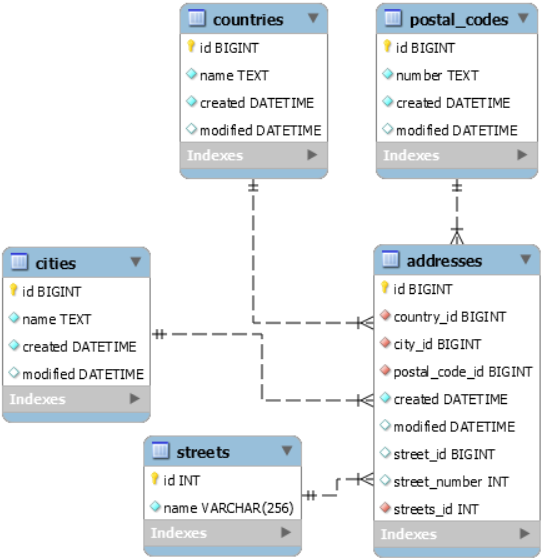
\includegraphics[width=0.8\textwidth]{addresses_diagram.png}
    \caption{Diagram modelu danych adresów. Opracowanie własne}
    \label{fig:diagram-adresy}
\end{figure}

Każda encja posiada unikalny identyfikator oraz kolumny opisujące czas utworzenia
oraz ewentualnej modyfikacji. Encja \textit{addresses} odwołuje się do pozostałych
encji za pomocą odpowiadających im identyfikatorów. 

Schemat adresów składa się z encji opisanych w tabeli \ref{tab:encje-adresow}:

    \begin{xltabular}{1\textwidth} { 
        | >{\raggedright\arraybackslash}c        
        | >{\raggedright\arraybackslash}X | }
        \caption{Encje w schemacie adresów} \label{tab:encje-adresow} \\
        \hline
       Nazwa encji & Przechowywane dane \\
       \hline
       Addresses & 
       Encja główna, zawiera odwołania do kraju, miasta, kodu pocztowego, numeru ulicy 
       oraz numeru budynku \\
       \hline
       Cities & Miasto \\
       \hline
       Countries & Kraj \\
       \hline
       Postal codes & Kod pocztowy \\
       \hline
       Streets & Ulica \\
       \hline
    \end{xltabular}

Związki między poszczególnymi encjami zostały opisane w tabeli \ref{tab:zwiazki-adresy}.
\newpage 

\begin{xltabular}{1\textwidth} { 
        | >{\arraybackslash}c    
        | >{\arraybackslash}c
        | >{\arraybackslash}c     
        | >{\arraybackslash}X | }
        \caption{Związki między encjami w schemacie adresów} \label{tab:zwiazki-adresy} \\
        \hline
    \multicolumn{2}{|c|}{Relacja} & Typ związku & Opis \\
    \hline
    Addresses & Countries & 1:N & 
    Każdy kraj może występować w wielu adresach \\
    \hline
    Addresses & Cities & 1:N & 
    Każde miasto może występować w wielu adresach \\
    \hline
    Addresses & Postal codes & 1:N 
    & Każdy kod pocztowy może występować w wielu adresach \\
    \hline
    Addresses & Strees & 1:N & 
    Każda ulica może występować w wielu adresach \\
    \hline
    \end{xltabular}

\subsubsection{Schemat organizacji}

Rysunek \ref{fig:diagram-organizacje} przedstawia diagram UML modelu danych organizacji. 

\begin{figure}[H]
    \centering
    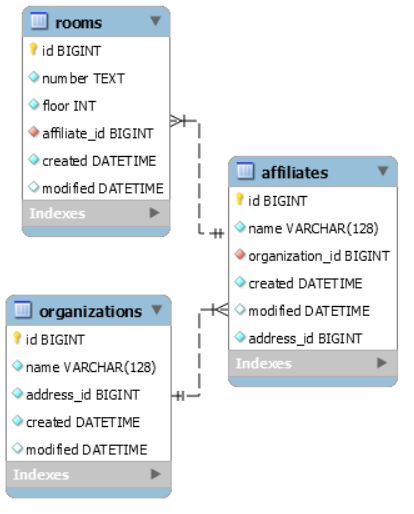
\includegraphics[width=0.7\textwidth]{facilities_diagram.png}
    \caption{Diagram modelu danych organizacji. Opracowanie własne}
    \label{fig:diagram-organizacje}
\end{figure}

Każda z encji posiada unikalny identyfikator oraz kolumny opisujące czas utworzenia
oraz ewentualnej modyfikacji. Oddziały są skojarzone z organizacjami poprzez
przechowywanie powiązanego z nią identyfikatora \textit{organization\_id}. Pomieszczenia natomiast powiązane
są z konkretnym oddziałem, również za pomocą stosownego identyfikatora \textit{affiliate\_id}.

Schemat organizacji składa się z encji opisanych w tabeli \ref{tab:encje-organizacji}:

    \begin{xltabular}{1\textwidth} { 
        | >{\raggedright\arraybackslash}c        
        | >{\raggedright\arraybackslash}X | }
        \caption{Encje w schemacie organizacji} \label{tab:encje-organizacji} \\
        \hline
       Nazwa encji & Przechowywane dane \\
       \hline
       Affiliates & 
       Oddziały danej organizacji \\
       \hline
       Rooms & Pomieszczenia w oddziałach \\
       \hline
       Organizations & Organizacje \\
       \hline
    \end{xltabular}

    Związki między poszczególnymi encjami zostały opisane w tabeli \ref{tab:zwiazki-organizacje}.


\begin{xltabular}{1\textwidth} { 
        | >{\arraybackslash}c   
        | >{\arraybackslash}c
        | >{\arraybackslash}c     
        | >{\arraybackslash}X | }
        \caption{Związki między encjami w schemacie organizacji} \label{tab:zwiazki-organizacje} \\
        \hline
    \multicolumn{2}{|c|}{Relacja} & Typ związku & Opis \\
    \hline
    Organizations & Affiliates & 1:N & 
    Każdy organizacja może posiadać wiele oddziałów \\
    \hline
    Affiliates & Rooms & 1:N & 
    Każdy oddział może posiadać wiele pomieszczeń \\
    \hline
    \end{xltabular}

\subsubsection{Schemat reguł}

Rysunek \ref{fig:diagram-reguly} przedstawia diagram UML modelu danych reguł. 
Każda z encji posiada unikalny identyfikator oraz kolumny opisujące czas utworzenia 
oraz ewentualnej modyfikacji. Encja \textit{expected\_room\_conditions} przechowuje
zestawy oczekiwanych warunków, jakie powinny panować w danym pomieszczeniu.
Poza konkretną wartością temperatury oraz natężenia światła określa się także
maksymalne tolerowane odchylenie wartości rzeczywistych od oczekiwanych.

Encja \textit{room\_policies} zawiera odwołanie do \textit{expected\_room\_conditions}
poprzez przechowywanie identyfikatora \textit{expected\_conditions\_id}.
Zawiera ona także daty, przechowywane w kolumnach \textit{start\_date} oraz 
\textit{end\_date} oraz oznaczające okres, w jakim dana reguła powinna obowiązywać.
Godziny obowiązywania zawarte są w kolumnach \textit{start\_hour} oraz \textit{end\_hour}.

Schemat reguł składa się z encji opisanych w tabeli \ref{tab:encje-regul}:
\newpage

\begin{figure}[H]
    \centering
    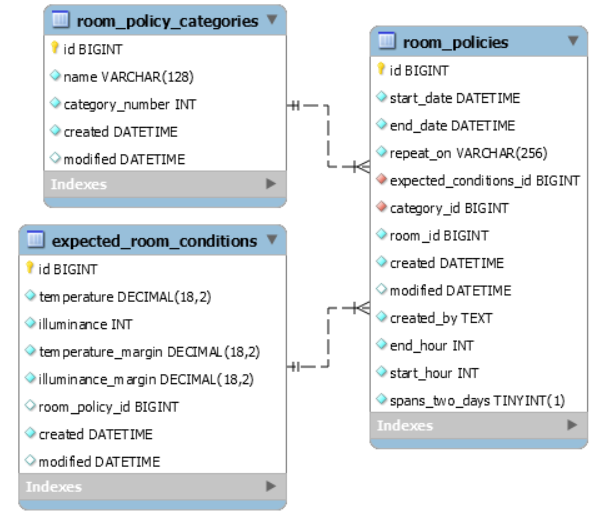
\includegraphics[width=0.8\textwidth]{policies_diagram.png}
    \caption{Diagram modelu danych reguł. Opracowanie własne}
    \label{fig:diagram-reguly}
\end{figure}

    \begin{xltabular}{1\textwidth} { 
        | >{\raggedright\arraybackslash}c        
        | >{\raggedright\arraybackslash}X | }
        \caption{Encje w schemacie reguł} \label{tab:encje-regul}\\
        \hline
       Nazwa encji & Przechowywane dane \\
       \hline
       Room policies & 
       Encja główna, zawiera odwołania do kategorii oraz oczekiwanych warunków. Przechowuje 
       okres obowiązywania danej reguły \\
       \hline
       Room policy categories & Kategorie reguł \\
       \hline
       Expected room conditions & Oczekiwane warunki w pomieszczeniu \\
       \hline
    \end{xltabular}



Związki między poszczególnymi encjami zostały opisane w tabeli \ref{tab:zwiazki-reguly}.
\newpage

\begin{xltabular}{1\textwidth} { 
        | >{\arraybackslash}c    
        | >{\arraybackslash}c
        | >{\arraybackslash}c     
        | >{\arraybackslash}X | }
        \caption{Związki między encjami w schemacie reguł} \label{tab:zwiazki-reguly} \\
        \hline
    \multicolumn{2}{|c|}{Relacja} & Typ związku & Opis \\
    \hline
    Room policies & Room policy categories & 1:N & 
    Każda kategoria może być przypisana wielu regułom \\
    \hline
    Room policies & Expected room conditions & 1:N & 
    Ten sam zbiór oczekiwanych warunków może być przypisany do wielu reguł \\
    \hline
    \end{xltabular}

\subsubsection{Schemat sensorów}

Rysunek \ref{fig:diagram-sensory} przedstawia diagram UML modelu danych sensorów. 

\begin{figure}[H]
    \centering
    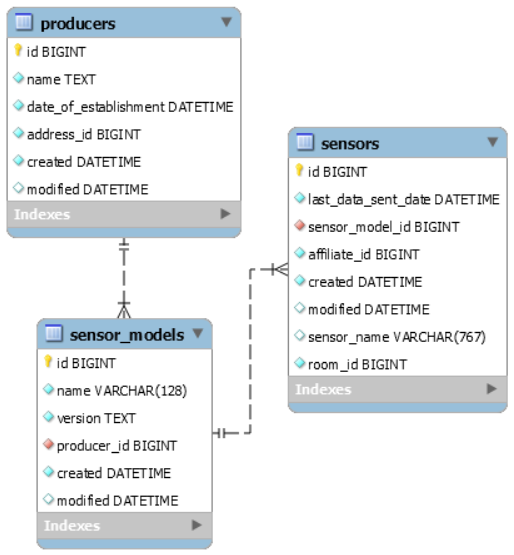
\includegraphics[width=0.8\textwidth]{sensors_diagram.png}
    \caption{Diagram modelu danych sensorów. Opracowanie własne}
    \label{fig:diagram-sensory}
\end{figure}

Każda z encji posiada unikalny identyfikator oraz kolumny opisujące czas utworzenia 
oraz ewentualnej modyfikacji. Producenci określają swoją nazwę oraz datę założenia
działalności. Produkują modele sensorów, które opisane są w encji 
\textit{sensor\_models}. Zawiera ona stosowny identyfikator \textit{producer\_id}
łączący obydwie encje. Każdy z modeli posiada własną nazwę oraz numer wersji.

Rekordy encji \textit{sensors} reprezentują kolejne instancje konkretnego modelu sensora.
Encje są ze sobą powiązane przy pomocy identyfikatora \textit{sensor\_model\_id}.
\textit{Sensors} zawiera także odwołania do oddziału oraz pomieszczenia, w którym
znajduje się urządzenie pomiarowe, przy użyciu identyfikatorów \textit{affiliate\_id}
oraz \textit{room\_id}.

Szczegółowe dane dotyczące oddziałów oraz pomieszczeń są przechowywane w schemacie
organizacji. Aby zachować niskie sprzężenie oraz wysoką spójność serwisów, wewnątrz
schematu sensorów należy się odwoływać do tych obiektów wyłącznie za pomocą unikalnego
identyfikatora. Nie powinno się także umieszczać dodatkowych kolumn opisujących
oddział lub pomieszczenie.

Schemat sensorów składa się z encji opisanych w tabeli \ref{tab:encje-sensorow}:

    \begin{xltabular}{1\textwidth} { 
        | >{\raggedright\arraybackslash}c        
        | >{\raggedright\arraybackslash}X | }
        \caption{Encje w schemacie sensorów} \label{tab:encje-sensorow} \\
        \hline
       Nazwa encji & Przechowywane dane \\
       \hline
       Sensors & Szczegóły dotyczące danego sensora \\
       \hline
       Sensor models & Model sensora \\
       \hline
       Producers & Producent sensorów \\
       \hline
    \end{xltabular}

Związki między poszczególnymi encjami zostały opisane w tabeli \ref{tab:zwiazki-sensory}.

\begin{xltabular}{1\textwidth} { 
        | >{\arraybackslash}c    
        | >{\arraybackslash}c
        | >{\arraybackslash}c     
        | >{\arraybackslash}X | }
        \caption{Związki między encjami w schemacie sensorów} \label{tab:zwiazki-sensory} \\
        \hline
    \multicolumn{2}{|c|}{Relacja} & Typ związku & Opis \\
    \hline
    Sensor models & Producers & 1:N & 
    Każdy producent może oferować wiele modeli sensorów \\
    \hline
    Sensor models & Sensors & 1:N & 
    Każdy model może być wypordukowany wielokrotnie \\
    \hline
    \end{xltabular}

    \newpage
\subsubsection{Schemat użytkowników}

Rysunek \ref{fig:diagram-uzytkownicy} przedstawia diagram UML modelu danych użytkowników. 

\begin{figure}[H]
    \centering
    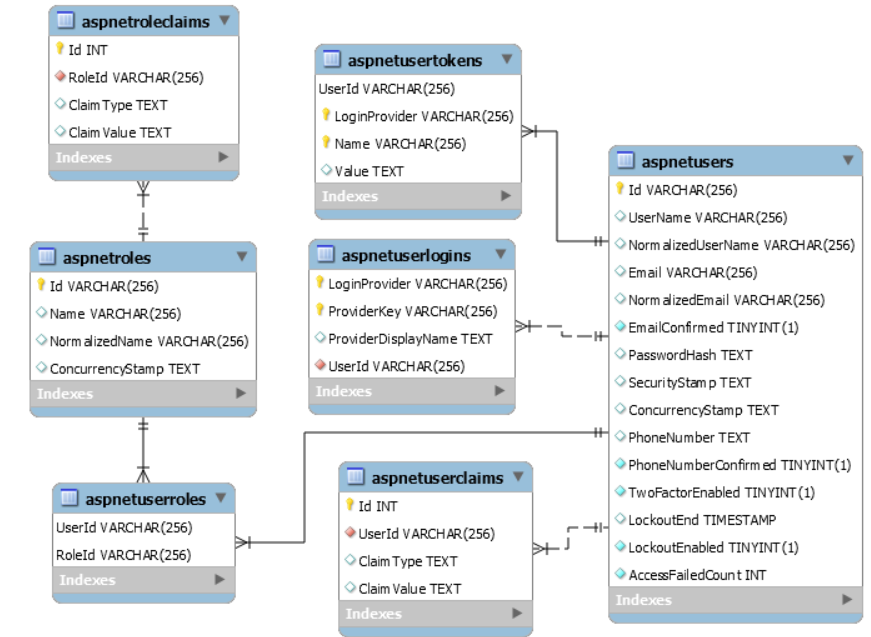
\includegraphics[width=1\textwidth]{users_diagram.png}
    \caption{Diagram modelu danych użytkowników. Opracowanie własne}
    \label{fig:diagram-uzytkownicy}
\end{figure}

Schemat użytkowników został oparty na schemacie oferowanym przez Microsoft 
\parencite{vickers2021} i składa się z następujących encji:

    \begin{xltabular}{1\textwidth} { 
        | >{\raggedright\arraybackslash}c        
        | >{\raggedright\arraybackslash}X | }
        \caption{Encje w schemacie użytkowników} \label{tab:encje-uzytkownicy}\\
        \hline
       Nazwa encji & Przechowywane dane \\
       \hline
       Asnetusers & Reprezentuje użytkownika \\
       \hline
       Aspnetroles & Reprezentuje rolę użytkownika w systemie \\
       \hline
       Aspnetuserlogins & Łączy użytkownika z loginem \\
       \hline
       Aspnetusertokens & Reprezentuje token uwierzytelniający dla użytkownika \\
       \hline
       Aspnetuserclaims & Reprezentuje prawa, które posiada użytkownik \\
       \hline
       Aspnetroleclaims & Reprezentuje prawa gwarantowane dla wszystkich użytkowników
       pełniących daną rolę \\
       \hline
       Aspnetuserroles & Łączy użytkowników z poszczególnymi rolami \\
       \hline
    \end{xltabular}

Związki między poszczególnymi encjami zostały opisane w tabeli \ref{tab:zwiazki-uzytkownicy}.

\begin{xltabular}{1\textwidth} { 
        | >{\arraybackslash}c    
        | >{\arraybackslash}c
        | >{\arraybackslash}c     
        | >{\arraybackslash}X | }
        \caption{Związki między encjami w schemacie użytkowników} \label{tab:zwiazki-uzytkownicy} \\
        \hline
    \multicolumn{2}{|c|}{Relacja} & Typ związku & Opis \\
    \hline
    Aspnetusers & Aspnetuserlogins & 1:N & 
    Każdemu użytkownikowi może być przypisanych wiele loginów \\
    \hline
    Aspnetusers & Aspnetusertokens & 1:N & 
    Każdemu użytkownikowi może być przypisanych wiele tokenów \\
    \hline
    Aspnetusers & Aspnetuserroles & 1:N &
    Każdy użytkownik może pełnić wiele ról \\
    \hline
    Aspnetusers & Aspnetuserclaims & 1:N &
    Każdy użytkownik może posiadać wiele praw \\
    \hline
    Aspnetroles & Aspnetroleclaims & 1:N &
    Każdej roli może być przypisanych wiele praw \\
    \hline
    Aspnetroles & Aspnetuserroles & 1:N &
    Każda rola może być pełniona przez wielu użytkowników \\
    \hline
    \end{xltabular}

\subsection{InfluxDB}
Sekcja opisuje sposób przechowywania
wykonanych przez czujniki pomiarów w bazie danych szeregów czasowych.

InfluxDB jest bazą danych szeregów czasowych służącą do przechowywania metryk 
i szeregów czasowych \cite{influxdb2022}. Umożliwia efektywne przechowywanie 
miliardów rekordów 
dzięki stosowaniu kompresji danych, oferuje także język zapytań pozwalający 
przeprowadzać kompleksowe analizy uzyskanych informacji. Dodatkową funkcjonalnością 
wyróżniającą tą bazę od standardowych relacyjnych baz danych jest możliwość 
zdefiniowania czasu, po którym rekordy będą usuwane. Można w ten sposób określić na 
przykład, że baza powinna przechowywać tylko rekordy z ostatniego miesiąca.

W niniejszej pracy baza danych szeregów czasowych została wykorzystana do 
przechowywania danych zbieranych z czujników temperatury oraz natężenia światła. 
Przychodzące informacje są zapisywane w kolejnych rekordach, które zawierają 
przedstawione w tabeli \ref{tab:parametry-pomiaru} parametry:

    \begin{xltabular}{1\textwidth} { 
        | >{\raggedright\arraybackslash}c 
        | >{\raggedright\arraybackslash}X | }
        \caption{Parametry pojedynczego rekordu przechowującego pomiar} \label{tab:parametry-pomiaru}\\
        \hline
       Parametr & Znaczenie \\
       \hline
       time & Czas otrzymania danych \\
       \hline
       field & Rodzaj danych \\
       \hline
       value & Zmierzona wartość \\
       \hline
    \end{xltabular}

    Domyślnie czas jest zapisywany z dokładnością do nanosekund. W tej pracy zostały
    zdefiniowane dwa rodzaje danych: \textit{temperature} dotyczące informacji o temperaturze 
    oraz \textit{illuminance} dotyczące informacji o natężeniu światła.
\newpage
\section{Komunikacja między mikroserwisami}
\label{section:komunikacja-miedzy-serwisami}

Sekcja przedstawia metody wykorzystane do przesyłania informacji między mikroserwisami.
Opisano rolę i różnice między brokerem wiadomości a stykami oferowanymi przez
poszczególne moduły usługowe. Podrozdział 6.1 przybliża szczegóły dotyczące zasad
działania brokera wiadomości. W podrozdziale 6.2 przedstawiono listę usług
oferowanych przez kolejne mikroserwisy.

\subsection{Broker wiadomości}
Sekcja opisuje wykorzystanie brokera wiadomości jako narzędzia do przekazywania
wiadomości między serwisami. Podrozdziały 6.1.1 oraz 6.1.2 prezentują szczegóły dotyczące
szyny danych oraz jej wykorzystania.

Aby mikroserwisy mogły działać poprawnie, potrzebują wymieniać ze sobą informacje 
w sposób szybki i niezawodny. W przypadku komunikacji nie wymagającej żadnej interakcji 
z użytkownikiem, jednym z rozwiązań jest wykorzystanie brokera wiadomości, który pełni 
rolę pośrednika przekazującego wiadomości między mikroserwisami. Do grona takich narzędzi 
należy RabbitMQ. Spośród konkurencyjnych rozwiązań wyróżnia się tym, że jest to 
narzędzie typu open source, ponadto cechuje się małymi wymaganiami sprzętowymi oraz 
łatwością wdrażania w chmurze. 

RabbitMQ wspiera różne protokoły do przekazywania wiadomości, jednak domyślnie 
wykorzystuje protokół AMQP 0-9-1 (ang. \textit{advanced message queuing protocol}). Uogólniony 
schemat, na którym opiera się protokół, został przedstawiony na rysunku \ref{fig:schemat-amqp}.

\begin{figure}[h]
    \centering
    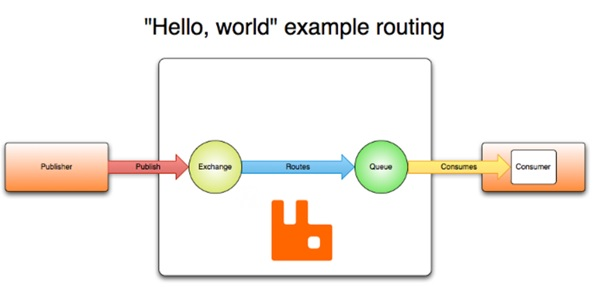
\includegraphics[width=1\textwidth]{amqp_schema.jpg}
    \caption{Schemat protokołu AMQP 0-9-1. Źródło: \cite{rabbitmq2022}}
    \label{fig:schemat-amqp}
\end{figure}

Wydawcy wiadomości (ang. \textit{publisher}) publikują wiadomości do pośrednika, który następnie 
je przekazuje do odpowiednich konsumentów (ang. \textit{consumer}). Ponieważ jest to protokół 
sieciowy, to wydawcy, konsumenci oraz pośrednicy mogą być uruchomieni na różnych 
maszynach. Pośrednik RabbitMQ działa według następujących zasad:

\begin{itemize} % lista nienumerowana
    \item Wiadomości są publikowane na giełdy (ang. exchange)
    \item Giełdy mogą być połączone z wieloma kolejkami (ang. \textit{queue})
    \item Zależnie od zastosowanej polityki kopia wiadomości może być przekazana do 
    każdej powiązanej kolejki lub tylko podzbiorowi kolejek
    \item Kolejka po otrzymaniu wiadomości od giełdy przesyła ją do konsumentów
\end{itemize}

Przesyłanie informacji przez sieć wiąże się z ryzykiem tego, że dane nie zostaną 
dostarczone. Wobec tego protokół zapewnia funkcjonalność zwaną potwierdzeniem 
wiadomości (ang. \textit{message acknowledgements}), która gwarantuje otrzymanie wiadomości 
przez konsumentów. Działa ona w ten sposób, że wiadomość jest usuwana z kolejki tylko 
wtedy, gdy uzyska potwierdzenie jej otrzymania od zainteresowanych mikrousług.

Giełdy po otrzymaniu wiadomości od wydawców mogą ją rozesłać do zera lub większej 
liczby kolejek. Używany algorytm routingu zależy od typu wymiany i reguł nazywanych 
powiązaniami (ang. \textit{bindings}). Pośrednicy korzystający z protokołu AMQP 0-9-1 zapewniają 
cztery typy wymiany:

\begin{itemize} % lista nienumerowana
    \item Wymiana bezpośrednia (ang. \textit{direct exchange}) - dostarcza wiadomości do kolejek 
    na podstawie klucza routingu. Jest idealna do wiadomości typu unicast 
    (chociaż może być także używana do wiadomości typu multicast)
    \item Wymiana do wszystkich (ang. \textit{fanout exchange}) - kieruje komunikaty do wszystkich 
    kolejek, które są z nią powiązane, a klucz routingu jest ignorowany. Jeśli do 
    giełdy dowiązanych jest N kolejek, to po publikacji wiadomości przez wydawcę 
    dotrze ona do wszystkich N kolejek. Jest idealna do rozsyłania wiadomości do 
    wszystkich konsumentów
    \item Wymiana tematyczna (ang. \textit{topic exchange}) - kieruje wiadomości do jednej lub 
    wielu kolejek na podstawie dopasowania klucza routingu oraz wzorca użytego do 
    powiązania kolejki z giełdą. Jest często używana do implementacji różnych odmian 
    wzorca publish/subscribe. Typowo używa się jej dla wiadomości typu multicast. 
    Warto ją rozważyć w przypadku, gdy należy dostarczyć wiadomość do wielu 
    konsumentów, które selektywnie wybierają rodzaj wiadomości, które chcą otrzymywać
    \item Wymiana nagłówków (ang. \textit{headers exchange}) - przeznaczona do routingu na 
    podstawie wielu atrybutów, które łatwiej można wyrazić w postaci nagłówków 
    wiadomości niż klucza routingu, który jest ignorowany. Wiadomość uważana jest za 
    zgodną i rozsyłana dalej, jeśli wartość nagłówka jest równa wartości określonej 
    podczas wiązania
\end{itemize}

AMQP 0-9-1 jest protokołem poziomu aplikacji, który używa protokołu TCP do niezawodnego 
przesyłania wiadomości. Połączenia (ang. \textit{connections}) korzystają z metod 
uwierzytelnienia i mogą być chronione za pomocą protokołu TLS. Ze względu na dodatkowe 
środki zapewniające niezawodność zaleca się, aby połączenia między klientem 
a pośrednikiem były ustanawiane na dłuższy okres czasu. W przypadku gdy klient 
potrzebuje nawiązać wiele połączeń, powinien wykorzystać kanały (ang. 
\textit{channels}), o których można myśleć jak o lekkich połączeniach dzielących jedno 
połączenie TCP. Każda operacja przeprowadzana przez klienta odbywa się z użyciem 
kanału, a komunikacja na różnych kanałach jest od siebie całkowicie odseparowana. 
Z tego względu każda metoda zawiera identyfikator kanału dla rozróżnienia, przez 
który kanał należy wysłać wiadomość.

\subsubsection{MassTransit}

Przy tworzeniu systemu została wykorzystana szyna danych o nazwie MassTransit 
przeznaczona dla aplikacji napisanych w modelu (ang. \textit{framework}) .NET Core
\cite{masstransit2022}. Zapewnia ona poziom 
abstrakcji umożliwiający wykorzystanie wielu różnych pośredników wiadomości, w 
tym RabbitMQ. Spośród wielu swoich zalet, szyna zapewnia:

\begin{itemize} % lista nienumerowana
    \item Równoczesne, asynchroniczne przetwarzanie wiadomości dla zwiększenia 
    przepustowości
    \item Zarządzanie połączeniem. Jeśli dany mikroserwis zostanie rozłączony 
    z pośrednikiem wiadomości, MassTransit spróbuje połączyć się ponownie oraz 
    przywrócić dotychczasowe giełdy, kolejki, a także połączenia między nimi
    \item Serializacja danych. Pośrednik wiadomości RabbitMq przesyła wiadomości 
    w postaci bajtów. Aby za jego pomocą przesłać obiekty specyficzne dla języka 
    C\#, trzeba zapisać je w odpowiednim formacie, w procesie zwanym serializacją. 
    MassTransit implementuje narzędzia do serializacji obiektów
    \item Testy jednostkowe. MassTransit zawiera implementację przygotowaną specjalnie 
    do testów w taki sposób, by testy nie były zależne od reszty infrastruktury 
    systemu. Przykładem jest poniższa metoda:
\end{itemize}

\begin{addmargin}[0mm]{10mm}
\begin{lstlisting}
    internal static async Task 
    PublishAndWaitToBeConsumed<T>(
        T @event, 
        InMemoryTestHarness testHarness)
    {
        var messageIdentifier = 
            await PublishMessage(@event, testHarness);

        var messageHasBeenConsumed = 
        await testHarness
            .Consumed
            .Any(x => 
            x.Context.MessageId == messageIdentifier);
        messageHasBeenConsumed.Should().BeTrue();

        var message = 
        await testHarness!
            .Consumed
            .SelectAsync(x => 
            x.Context.MessageId == messageIdentifier)
            .First();

        message.Exception.Should()
            .BeNull(
                "Message has been consumed 
                without any errors");
    }
    \end{lstlisting}
\end{addmargin}

Metoda publikuje testową wiadomość, po czym sprawdza, czy została prawidłowo 
przetworzona. 

Dzięki zastosowaniu szyny danych tworzenie konsumentów oraz publikowanie wiadomości 
staje się dużo łatwiejsze. Aby utworzyć nowego konsumenta, wystarczy jedynie utworzyć 
nową klasę implementującą interfejs \textit{IConsumer<T>}, gdzie \textit{T} jest oczekiwanym typem 
wiadomości. Klasa musi zawierać implementację metody 
\textit{Consume(ConsumeContext<MeasurementSentEvent> context)}, która zawiera logikę 
przetwarzania wiadomości. Przykładem jest poniższa metoda:

\begin{addmargin}[0mm]{10mm}
\begin{lstlisting}
    public async Task Consume(
        ConsumeContext<MeasurementSentEvent> context)
    {
        var policiesEvaluationResultEvent = 
        await _evaluatePoliciesCommand
            .Handle(context.Message);

        await _eventPublisher
            .Publish(policiesEvaluationResultEvent);
        _logger.LogInformation(
            $"PoliciesEvaluationResultEvent sent 
            from PolicyNode. Message: 
            {policiesEvaluationResultEvent.Message}");
    }

    \end{lstlisting}
\end{addmargin}
    
Zapisuje ona w logach szczegóły dotyczące przychodzącej wiadomości, przetwarza 
otrzymane wartości, po czym publikuje nową wiadomość o innym typie, której konsument 
jest implementowany przez inny mikroserwis.

\subsubsection{Połączenie mikroserwisów z brokerem wiadomości}

Utworzone w ramach pracy mikroserwisy łączą się z brokerem wiadomości i w ten sposób wymieniają między
sobą dane. Mogą one być połączone w różny sposób, zależnie od oczekiwanego rezultatu. Dwa główne
przypadki zostały przedstawione na rysunku \ref{fig:rabbitmq-polaczenie}.

\begin{figure}[h]
    \centering
    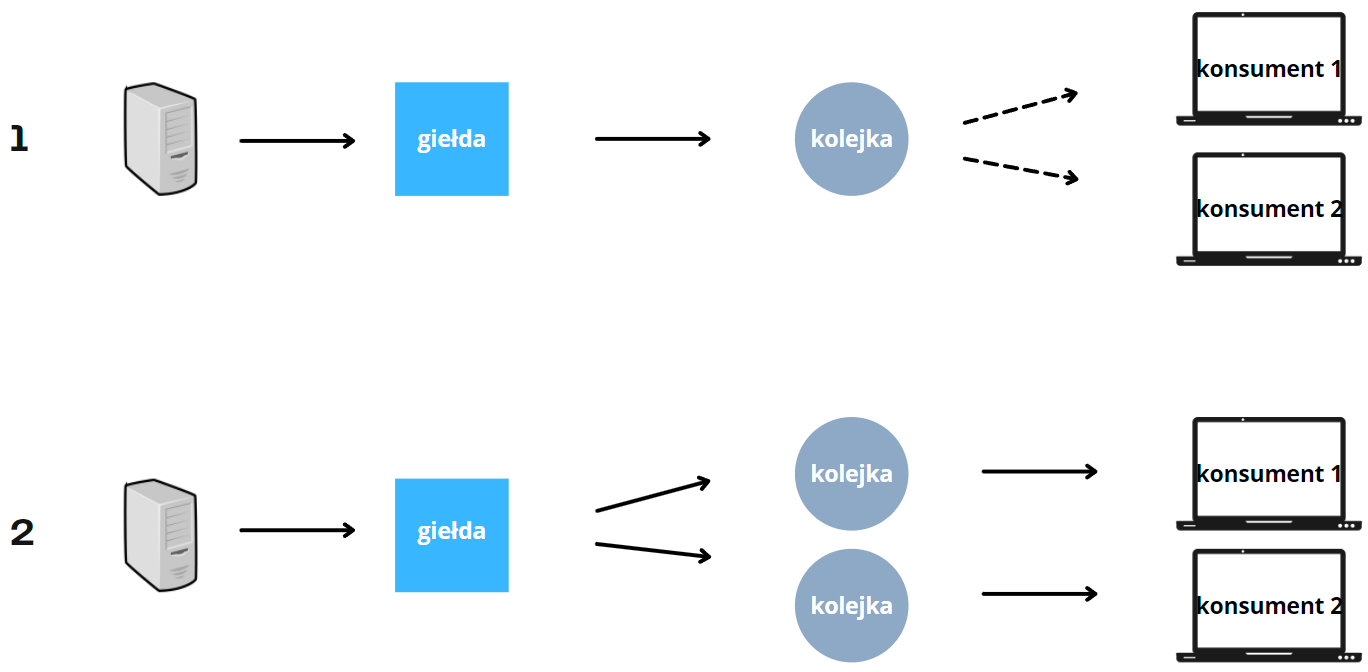
\includegraphics[width=1\textwidth]{rabbitmq_schema.jpg}
    \caption{Rodzaje połączenia z brokerem wiadomości. Opracowanie własne}
    \label{fig:rabbitmq-polaczenie}
\end{figure}

\begin{enumerate}
    \item W pierwszym przypadku celem jest wysłanie wiadomości tylko do jednego konsumenta. Jedną
    z występujących sytuacji jest przetwarzanie otrzymanych z czujników pomiarów przez SSPS. 
    Wykonanie tej samej operacji przez kilka instancji tego serwisu byłoby stratą
    dostępnych zasobów. Aby osiągnąć ten efekt, wszystkie instancje tego serwisu powinny być dołączone 
    do jednej kolejki. Wtedy kolejka wysyła przychodzące pomiary tylko do wybranej przez siebie instancji.
    Wybór odbywa się za pomocą mechanizmu szeregowania procesów Round-robin.
    \item W drugim przypadku celem jest wysłanie wiadomości do wielu konsumentów. Jedną z występujących
    sytuacji jest wysłanie wyniku przetwarzania pomiarów do wszystkich pracowników oraz administratorów
    posiadających uprawnienia do jego wyświetlenia. Aby osiągnąć ten efekt, każda instancja serwisów
    otrzymujących wynik (w tym wypadku są to AAS oraz EAS)
    powinna być dołączona do osobnej kolejki, z których wszystkie dołączone są do tej samej giełdy
    publikującej wiadomości. W ten sposób kopia wysłanej przez wydawcę wiadomości zostanie dostarczona
    do każdej instancji.
\end{enumerate}

\subsection{Styki}
Sekcja przedstawia opis styków jako narzędzia do komunikacji między serwisami.
W podrozdziałach 6.2.1 - 6.2.5 przedstawiono
listę udostępnianych przez kolejne mikroserwisy usług, ich wymagane parametry wejściowe
oraz rodzaj zwracanej odpowiedzi.

Mikroserwisy mogą komunikować się między sobą przy użyciu oferowanych przez nie 
styków (ang. \textit{Application Programming Interface}). Definiują parametry wymagane 
do realizacji usługi oraz zbiór danych zwracany w odpowiedzi.

Mikrousługi aplikacyjne oraz mikrousługi danych oferują styki zwracające jasno 
zdefiniowany zbiór danych. Zostały one szczegółowo opisane w poniższych podrozdziałach. 
Każda z oferowanych usług zawiera:

\begin{itemize} % lista nienumerowana
    \item Krótki opis funkcjonalności
    \item Wykorzystywany czasownik protokołu http. Jeden z GET, POST, UPDATE, DELETE
    \item wymagane parametry wejściowe
    \item numer statusu oraz typ zwracanego obiektu
\end{itemize}

\subsubsection{Usługi udostępniane przez mikrousługę danych adresów}

ADS oferuje usługi zwracające szczegółowe dane dotyczące adresów oraz pozwalające
na ich manipulację.

\begin{xltabular}{1\textwidth} { 
        | c    
        | c
        | X | }
        \caption{Usługi udostępniane przez ADS} \label{tab:styki-addresses} \\
        \hline
    \textbf{Ścieżka} & 
    \multicolumn{2}{c|}{GET /addresses-api/addresses/\{addressId\}} \\
    \hline
    \textbf{Opis} & 
    \multicolumn{2}{c|}{\makecell{Zwraca informacje na temat adresu o danym identyfikatorze}} \\    \hline
    \textbf{Odpowiedź} &
    \textbf{Kod odpowiedzi} &
    \textbf{Schemat} \\
    \hline
    {} & 200 & AddressDtoJsonApiDocument \\
    \hline
    {} & 404 & JsonApiError \\
    \hline
    \hline
    \hline
    \textbf{Ścieżka} & 
    \multicolumn{2}{c|}{POST /addresses-api/addresses} \\
    \hline
    \textbf{Opis} & 
    \multicolumn{2}{c|}{\makecell{Tworzy nowy adres o parametrach podanych \\ w modelu AddNewAddressCommand}} \\    \hline
    \textbf{Odpowiedź} &
    \textbf{Kod odpowiedzi} &
    \textbf{Schemat} \\
    \hline
    {} & 201 & AddressDtoJsonApiDocument \\
    \hline
    {} & 400 & JsonApiError \\
    \hline
    \hline
    \hline
    \textbf{Ścieżka} & 
    \multicolumn{2}{c|}{GET /addresses-api/cities/\{cityId\}} \\
    \hline
    \textbf{Opis} & 
    \multicolumn{2}{c|}{\makecell{Zwraca informacje na temat miasta o danym identyfikatorze}} \\    \hline
    \textbf{Odpowiedź} &
    \textbf{Kod odpowiedzi} &
    \textbf{Schemat} \\
    \hline
    {} & 200 & CityDtoJsonApiDocument \\
    \hline
    {} & 404 & JsonApiError \\
    \hline
    \hline
    \hline
    \textbf{Ścieżka} & 
    \multicolumn{2}{c|}{GET /addresses-api/countries/\{countryId\}} \\
    \hline
    \textbf{Opis} & 
    \multicolumn{2}{c|}{\makecell{Zwraca informacje na temat kraju o danym identyfikatorze}} \\    \hline
    \textbf{Odpowiedź} &
    \textbf{Kod odpowiedzi} &
    \textbf{Schemat} \\
    \hline
    {} & 200 & CountryDtoJsonApiDocument \\
    \hline
    {} & 404 & JsonApiError \\
    \hline
    \hline
    \hline
    \textbf{Ścieżka} & 
    \multicolumn{2}{c|}{GET /addresses-api/postal-codes/\{postalCodeId\}} \\
    \hline
    \textbf{Opis} & 
    \multicolumn{2}{c|}{\makecell{Zwraca informacje na temat kodu \\pocztowego o danym identyfikatorze}} \\    \hline
    \textbf{Odpowiedź} &
    \textbf{Kod odpowiedzi} &
    \textbf{Schemat} \\
    \hline
    {} & 200 & PostalCodeDtoJsonApiDocument \\
    \hline
    {} & 404 & JsonApiError \\
    \hline
    \end{xltabular}

\subsubsection{Usługi udostępniane przez mikrousługę danych organizacji}
FDS udostępnia zbiór usług pozwalających na zarządzanie przechowywanymi informacjami
o organizacjach, oddziałach oraz pomieszczeniach. 

    
\begin{xltabular}{1\textwidth} { 
        | c    
        | c
        | X | }
        \caption{Usługi udostępniane przez FDS} \label{tab:styki-facilities} \\
        \hline
    \textbf{Ścieżka} & 
    \multicolumn{2}{c|}{GET /facilities-api/affiliates/\{affiliateId\}} \\
    \hline
    \textbf{Opis} & 
    \multicolumn{2}{c|}{\makecell{Zwraca informacje na temat oddziału o danym identyfikatorze}} \\    \hline
    \textbf{Odpowiedź} &
    \textbf{Kod odpowiedzi} &
    \textbf{Schemat} \\
    \hline
    {} & 200 & AffiliateDtoJsonApiDocument \\
    \hline
    {} & 404 & JsonApiError \\
    \hline
    \hline
    \hline
    \textbf{Ścieżka} & 
    \multicolumn{2}{c|}{DELETE /facilities-api/affiliates/\{affiliateId\}} \\
    \hline
    \textbf{Opis} & 
    \multicolumn{2}{c|}{\makecell{Usuwa informacje na temat oddziału o danym identyfikatorze}} \\    \hline
    \textbf{Odpowiedź} &
    \textbf{Kod odpowiedzi} &
    \textbf{Schemat} \\
    \hline
    {} & 204 & Brak zawartości \\
    \hline
    {} & 404 & JsonApiError \\
    \hline
    \hline
    \hline
    \textbf{Ścieżka} & 
    \multicolumn{2}{c|}{POST /facilities-api/organizations} \\
    \hline
    \textbf{Opis} & 
    \multicolumn{2}{c|}{\makecell{Tworzy nową organizację o parametrach podanych \\w modelu AddNewOrganizationCommand}} \\    \hline
    \textbf{Odpowiedź} &
    \textbf{Kod odpowiedzi} &
    \textbf{Schemat} \\
    \hline
    {} & 201 & OrganizationDtoJsonApiDocument \\
    \hline
    {} & 400 & JsonApiError \\
    \hline
    {} & 409 & JsonApiError \\
    \hline
    \hline
    \hline
    \textbf{Ścieżka} & 
    \multicolumn{2}{c|}{GET /facilities-api/organizations} \\
    \hline
    \textbf{Opis} & 
    \multicolumn{2}{c|}{\makecell{Zwraca informacje na temat wszystkich organizacji}} \\    \hline
    \textbf{Odpowiedź} &
    \textbf{Kod odpowiedzi} &
    \textbf{Schemat} \\
    \hline
    {} & 200 & OrganizationDtoListJsonApiDocument \\
    \hline
    \hline
    \hline
    \textbf{Ścieżka} & 
    \multicolumn{2}{c|}{GET /facilities-api/organizations/\{organizationId\}} \\
    \hline
    \textbf{Opis} & 
    \multicolumn{2}{c|}{\makecell{Zwraca informacje na temat organizacji o danym identyfikatorze}} \\    \hline
    \textbf{Odpowiedź} &
    \textbf{Kod odpowiedzi} &
    \textbf{Schemat} \\
    \hline
    {} & 200 & OrganizationDtoJsonApiDocument \\
    \hline
    {} & 404 & JsonApiError \\
    \hline
    \hline
    \hline
    \textbf{Ścieżka} & 
    \multicolumn{2}{c|}{DELETE /facilities-api/organizations/\{organizationId\}} \\
    \hline
    \textbf{Opis} & 
    \multicolumn{2}{c|}{\makecell{Usuwa informacje na temat organizacji o danym identyfikatorze}} \\    \hline
    \textbf{Odpowiedź} &
    \textbf{Kod odpowiedzi} &
    \textbf{Schemat} \\
    \hline
    {} & 204 & Brak zawartości \\
    \hline
    {} & 404 & JsonApiError \\
    \hline
    \hline
    \hline
    \textbf{Ścieżka} & 
    \multicolumn{2}{c|}{POST /facilities-api/rooms} \\
    \hline
    \textbf{Opis} & 
    \multicolumn{2}{c|}{\makecell{Tworzy nowe pomieszczenie o parametrach podanych \\w modelu AddNewRoomCommand}} \\    \hline
    \textbf{Odpowiedź} &
    \textbf{Kod odpowiedzi} &
    \textbf{Schemat} \\
    \hline
    {} & 201 & RoomDtoJsonApiDocument \\
    \hline
    {} & 400 & JsonApiError \\
    \hline
    {} & 409 & JsonApiError \\
    \hline
    \hline
    \hline
    \textbf{Ścieżka} & 
    \multicolumn{2}{c|}{GET /facilities-api/rooms/\{roomId\}} \\
    \hline
    \textbf{Opis} & 
    \multicolumn{2}{c|}{\makecell{Zwraca informacje na temat pomieszczenia o danym identyfikatorze}} \\    \hline
    \textbf{Odpowiedź} &
    \textbf{Kod odpowiedzi} &
    \textbf{Schemat} \\
    \hline
    {} & 200 & RoomDtoJsonApiDocument \\
    \hline
    {} & 404 & JsonApiError \\
    \hline
    \hline
    \hline
    \textbf{Ścieżka} & 
    \multicolumn{2}{c|}{DELETE /facilities-api/rooms/\{roomId\}} \\
    \hline
    \textbf{Opis} & 
    \multicolumn{2}{c|}{\makecell{Usuwa informacje na temat pomieszczenia o danym identyfikatorze}} \\    \hline
    \textbf{Odpowiedź} &
    \textbf{Kod odpowiedzi} &
    \textbf{Schemat} \\
    \hline
    {} & 204 & Brak zawartości \\
    \hline
    {} & 404 & JsonApiError \\
    \hline
    \hline
    \hline
    \end{xltabular}

\subsubsection{Usługi udostępniane przez mikrousługę danych reguł}
Usługi oferowane przez PDS pozwalają na zwracanie informacji dotyczących 
istniejących reguł, a także dodawanie nowych rekordów o różnych typach reguł. 
    
\begin{xltabular}{1\textwidth} { 
        | c    
        | c
        | X | }
        \caption{Usługi udostępniane przez PDS} \label{tab:reguly-styki} \\
        \hline
    \textbf{Ścieżka} & 
    \multicolumn{2}{c|}{POST /policies-api/expected-room-conditions} \\
    \hline
    \textbf{Opis} & 
    \multicolumn{2}{c|}{\makecell{Tworzy nowy zestaw oczekiwanych wartości mierzonych\\parametrów określonych w modelu \\AddNewExpectedRoomConditionsCommand}} \\    \hline
    \textbf{Odpowiedź} &
    \textbf{Kod odpowiedzi} &
    \textbf{Schemat} \\
    \hline
    {} & 201 & OrganizationDtoJsonApiDocument \\
    \hline
    {} & 400 & JsonApiError \\
    \hline
    \hline
    \hline
    \textbf{Ścieżka} & 
    \multicolumn{2}{c|}{\makecell{GET /policies-api/expected-room-\\conditions/\{expectedRoomConditionsId\}}} \\
    \hline
    \textbf{Opis} & 
    \multicolumn{2}{c|}{\makecell{Zwraca informacje na temat zestawu oczekiwanych wartości\\mierzonych parametrów o danym identyfikatorze}} \\    \hline
    \textbf{Odpowiedź} &
    \textbf{Kod odpowiedzi} &
    \textbf{Schemat} \\
    \hline
    {} & 200 & RoomDtoJsonApiDocument \\
    \hline
    {} & 404 & JsonApiError \\
    \hline
    \hline
    \hline
    \textbf{Ścieżka} & 
    \multicolumn{2}{c|}{POST /policies-api/policies} \\
    \hline
    \textbf{Opis} & 
    \multicolumn{2}{c|}{\makecell{Tworzy nową regułę o parametrach określonych \\w modelu AddNewRoomPolicyCommand}} \\    \hline
    \textbf{Odpowiedź} &
    \textbf{Kod odpowiedzi} &
    \textbf{Schemat} \\
    \hline
    {} & 201 & RoomPolicyDtoJsonApiDocument \\
    \hline
    {} & 400 & JsonApiError \\
    \hline
    \hline
    \hline
    \textbf{Ścieżka} & 
    \multicolumn{2}{c|}{POST /policies-api/policies/past-policies} \\
    \hline
    \textbf{Opis} & 
    \multicolumn{2}{c|}{\makecell{Zwraca listę reguł poprzednio obowiązujących \\w pomieszczeniu określonym w modelu GetPastPoliciesCommand}} \\    \hline
    \textbf{Odpowiedź} &
    \textbf{Kod odpowiedzi} &
    \textbf{Schemat} \\
    \hline
    {} & 201 & PastMeasurementsDtoJsonApiDocument \\
    \hline
    {} & 400 & JsonApiError \\
    \hline
    \hline
    \hline
    \textbf{Ścieżka} & 
    \multicolumn{2}{c|}{GET /policies-api/policies/\{roomId\}} \\
    \hline
    \textbf{Opis} & 
    \multicolumn{2}{c|}{\makecell{Zwraca informacje na temat aktualnie obowiązującej \\polityki w pomieszczeniu o danym identyfikatorze}} \\    \hline
    \textbf{Odpowiedź} &
    \textbf{Kod odpowiedzi} &
    \textbf{Schemat} \\
    \hline
    {} & 200 & RoomPolicyDtoJsonApiDocument \\
    \hline
    {} & 404 & JsonApiError \\
    \hline
    \end{xltabular}

\subsubsection{Usługi udostępniane przez mikrousługę danych sensorów}
SDS udostępnia usługi pozwalające na uzyskiwanie informacji o istniejących
sensorach oraz dodawanie nowych rekordów.
    
\begin{xltabular}{1\textwidth} { 
        | c    
        | c
        | X | }
        \caption{Usługi udostępniane przez SDS} \label{tab:sensory-styki} \\
        \hline
    \textbf{Ścieżka} & 
    \multicolumn{2}{c|}{GET /sensors-api/sensors} \\
    \hline
    \textbf{Opis} & 
    \multicolumn{2}{c|}{\makecell{Zwraca informacje na temat wszystkich sensorów}} \\    \hline
    \textbf{Odpowiedź} &
    \textbf{Kod odpowiedzi} &
    \textbf{Schemat} \\
    \hline
    {} & 200 & SensorDtoListJsonApiDocument \\
    \hline
    \hline
    \hline
    \textbf{Ścieżka} & 
    \multicolumn{2}{c|}{GET /sensors-api/sensors/room-id/\{roomId\}} \\
    \hline
    \textbf{Opis} & 
    \multicolumn{2}{c|}{\makecell{Zwraca informacje na temat sensorów znajdujących się \\w pomieszczeniu o danym identyfikatorze}} \\    \hline
    \textbf{Odpowiedź} &
    \textbf{Kod odpowiedzi} &
    \textbf{Schemat} \\
    \hline
    {} & 200 & SensorDtoJsonApiDocument \\
    \hline
    {} & 404 & JsonApiError \\
    \hline
    \hline
    \hline
    \textbf{Ścieżka} & 
    \multicolumn{2}{c|}{POST /sensors-api/sensors/sensor-name} \\
    \hline
    \textbf{Opis} & 
    \multicolumn{2}{c|}{\makecell{Zwraca informacje na temat sensorów o parametrach \\określonych w modelu GetSensorBySensorNameCommand}} \\    \hline
    \textbf{Odpowiedź} &
    \textbf{Kod odpowiedzi} &
    \textbf{Schemat} \\
    \hline
    {} & 200 & SensorDtoJsonApiDocument \\
    \hline
    {} & 400 & JsonApiError \\
    \hline
    \hline
    \hline
    \textbf{Ścieżka} & 
    \multicolumn{2}{c|}{GET /sensors-api/sensors/\{sensorId\}} \\
    \hline
    \textbf{Opis} & 
    \multicolumn{2}{c|}{\makecell{Zwraca informacje na temat sensorów o danym identyfikatorze}} \\    \hline
    \textbf{Odpowiedź} &
    \textbf{Kod odpowiedzi} &
    \textbf{Schemat} \\
    \hline
    {} & 200 & SensorDtoJsonApiDocument \\
    \hline
    {} & 404 & JsonApiError \\
    \hline
    \end{xltabular}

\subsubsection{Usługi udostępniane przez mikrousługę aplikacyjną administratorów}
Usługi udostępniane przez AAS pozwalają na uzyskiwanie danych dotyczących organizacji,
oddziałów i pomieszczeń, a także na ich dodawanie.

\begin{xltabular}{1\textwidth} { 
        | c    
        | c
        | X | }
        \caption{Usługi udostępniane przez AAS} \label{tab:admin-styki} \\
        \hline
    \textbf{Ścieżka} & 
    \multicolumn{2}{c|}{POST /admin-node/addresses} \\
    \hline
    \textbf{Opis} & 
    \multicolumn{2}{c|}{\makecell{Tworzy nowy adres o parametrach określonych \\w modelu AddNewAddressCommand}} \\    \hline
    \textbf{Odpowiedź} &
    \textbf{Kod odpowiedzi} &
    \textbf{Schemat} \\
    \hline
    {} & 201 & AddressDtoJsonApiDocument \\
    \hline
    {} & 400 & JsonApiError \\
    \hline
    \hline
    \hline
    \textbf{Ścieżka} & 
    \multicolumn{2}{c|}{POST /admin-node/affiliates} \\
    \hline
    \textbf{Opis} & 
    \multicolumn{2}{c|}{\makecell{Tworzy nowy oddział o parametrach określonych \\w modelu AddNewAffiliateCommand}} \\    \hline
    \textbf{Odpowiedź} &
    \textbf{Kod odpowiedzi} &
    \textbf{Schemat} \\
    \hline
    {} & 201 & AffiliateDtoJsonApiDocument \\
    \hline
    {} & 400 & JsonApiError \\
    \hline
    {} & 409 & JsonApiError \\
    \hline
    \hline
    \hline
    \textbf{Ścieżka} & 
    \multicolumn{2}{c|}{GET /admin-node/affiliates} \\
    \hline
    \textbf{Opis} & 
    \multicolumn{2}{c|}{\makecell{Zwraca informacje na temat wszystkich oddziałów}} \\    \hline
    \textbf{Odpowiedź} &
    \textbf{Kod odpowiedzi} &
    \textbf{Schemat} \\
    \hline
    {} & 200 & AdminNodeAffiliateDtoListJsonApiDocument \\
    \hline
    {} & 404 & JsonApiError \\
    \hline
    \hline
    \hline
    \textbf{Ścieżka} & 
    \multicolumn{2}{c|}{GET /admin-node/affiliates/\{affiliateId\}} \\
    \hline
    \textbf{Opis} & 
    \multicolumn{2}{c|}{\makecell{Zwraca informacje na temat oddziału o danym identyfikatorze}} \\    \hline
    \textbf{Odpowiedź} &
    \textbf{Kod odpowiedzi} &
    \textbf{Schemat} \\
    \hline
    {} & 200 & AdminNodeAffiliateDtoJsonApiDocument \\
    \hline
    {} & 404 & JsonApiError \\
    \hline
    \hline
    \hline
    \textbf{Ścieżka} & 
    \multicolumn{2}{c|}{DELETE /admin-node/affiliates/\{affiliateId\}} \\
    \hline
    \textbf{Opis} & 
    \multicolumn{2}{c|}{\makecell{Usuwa informacje na temat oddziału o danym identyfikatorze}} \\    \hline
    \textbf{Odpowiedź} &
    \textbf{Kod odpowiedzi} &
    \textbf{Schemat} \\
    \hline
    {} & 204 & Brak zawartości \\
    \hline
    {} & 404 & JsonApiError \\
    \hline
    \hline
    \hline
    \textbf{Ścieżka} & 
    \multicolumn{2}{c|}{POST /admin-node/organizations} \\
    \hline
    \textbf{Opis} & 
    \multicolumn{2}{c|}{\makecell{Tworzy nową organizację o parametrach określonych \\w modelu AddNewOrganizationCommand}} \\    \hline
    \textbf{Odpowiedź} &
    \textbf{Kod odpowiedzi} &
    \textbf{Schemat} \\
    \hline
    {} & 201 & OrganizationDtoJsonApiDocument \\
    \hline
    {} & 400 & JsonApiError \\
    \hline
    {} & 409 & JsonApiError \\
    \hline
    \hline
    \hline
    \textbf{Ścieżka} & 
    \multicolumn{2}{c|}{GET /admin-node/organizations} \\
    \hline
    \textbf{Opis} & 
    \multicolumn{2}{c|}{\makecell{Zwraca informacje na temat wszystkich organizacji}} \\    \hline
    \textbf{Odpowiedź} &
    \textbf{Kod odpowiedzi} &
    \textbf{Schemat} \\
    \hline
    {} & 200 & \makecell{AdminNodeOrganizationDto\\ListJsonApiDocument} \\
    \hline
    {} & 404 & JsonApiError \\
    \hline
    \hline
    \hline
    \textbf{Ścieżka} & 
    \multicolumn{2}{c|}{GET /admin-node/organizations/\{organizationId\}} \\
    \hline
    \textbf{Opis} & 
    \multicolumn{2}{c|}{\makecell{Zwraca informacje na temat organizacji o danym identyfikatorze}} \\    \hline
    \textbf{Odpowiedź} &
    \textbf{Kod odpowiedzi} &
    \textbf{Schemat} \\
    \hline
    {} & 200 & \makecell{AdminNodeOrganizationDto\\ListJsonApiDocument} \\
    \hline
    {} & 404 & JsonApiError \\
    \hline
    \hline
    \hline
    \textbf{Ścieżka} & 
    \multicolumn{2}{c|}{DELETE /admin-node/organizations/\{organizationId\}} \\
    \hline
    \textbf{Opis} & 
    \multicolumn{2}{c|}{\makecell{Usuwa informacje na temat organizacji o danym identyfikatorze}} \\    \hline
    \textbf{Odpowiedź} &
    \textbf{Kod odpowiedzi} &
    \textbf{Schemat} \\
    \hline
    {} & 204 & Brak zawartości \\
    \hline
    {} & 404 & JsonApiError \\
    \hline
    \hline
    \hline
    \textbf{Ścieżka} & 
    \multicolumn{2}{c|}{POST /admin-node/rooms} \\
    \hline
    \textbf{Opis} & 
    \multicolumn{2}{c|}{\makecell{Tworzy nowe pomieszczenie o parametrach określonych \\w modelu AddNewRoomCommand}} \\    \hline
    \textbf{Odpowiedź} &
    \textbf{Kod odpowiedzi} &
    \textbf{Schemat} \\
    \hline
    {} & 201 & RoomDtoJsonApiDocument \\
    \hline
    {} & 400 & JsonApiError \\
    \hline
    {} & 409 & JsonApiError \\
    \hline
    \hline
    \hline
    \textbf{Ścieżka} & 
    \multicolumn{2}{c|}{POST /admin-node/rooms/get-room} \\
    \hline
    \textbf{Opis} & 
    \multicolumn{2}{c|}{\makecell{Zwraca informacje o pomieszczeniu o parametrach podanych \\w modelu GetRoomCommand}} \\    \hline
    \textbf{Odpowiedź} &
    \textbf{Kod odpowiedzi} &
    \textbf{Schemat} \\
    \hline
    {} & 200 & 	
    AdminNodeRoomDtoJsonApiDocument \\
    \hline
    {} & 404 & JsonApiError \\
    \hline
    \hline
    \hline
    \textbf{Ścieżka} & 
    \multicolumn{2}{c|}{POST /admin-node/rooms/historic-measurements} \\
    \hline
    \textbf{Opis} & 
    \multicolumn{2}{c|}{\makecell{Zwraca informacje o historycznych pomiarach z pomieszczenia \\o parametrach podanych w modelu GetRoomCommand}} \\    \hline
    \textbf{Odpowiedź} &
    \textbf{Kod odpowiedzi} &
    \textbf{Schemat} \\
    \hline
    {} & 200 & 	
    PastMeasurementsDtoJsonApiDocument \\
    \hline
    {} & 400 & JsonApiError \\
    \hline
    \hline
    \hline
    \textbf{Ścieżka} & 
    \multicolumn{2}{c|}{DELETE /admin-node/rooms/\{roomId\}} \\
    \hline
    \textbf{Opis} & 
    \multicolumn{2}{c|}{\makecell{Usuwa informacje na temat pomieszczenia o danym identyfikatorze}} \\    \hline
    \textbf{Odpowiedź} &
    \textbf{Kod odpowiedzi} &
    \textbf{Schemat} \\
    \hline
    {} & 204 & Brak zawartości \\
    \hline
    {} & 404 & JsonApiError \\
    \hline
    \end{xltabular}
\newpage
\section{Testy}
Sekcja opisuje wykorzystane rodzaje testów oraz przedstawia przypadki ich użycia.
Podrozdział 7.1 prezentuje szczegóły dotyczące testów jednostkowych oraz
przedstawia argumenty przekonujące do zapewnienia dużej liczby tego rodzaju testów.
W podrozdziale 7.2 opisano rolę testów integracyjnych. Poprawność funkcji biznesowych
można sprawdzić dzięki testom typu end-2-end, przybliżonych w podrozdziale 7.3.
Proces przeprowadzania testów można zautomatyzować przy pomocy narzędzi opisanych
w podrozdziale 7.4

Dobrą praktyką pozwalającą znacznie ograniczyć występowanie błędów w ostatecznej 
wersji systemu jest przygotowanie testów sprawdzających działanie poszczególnych 
funkcji. Istnieje kilka rodzajów testów, które można pogrupować tak jak na rysunku
\ref{fig:test-types}.

\begin{figure}[h]
    \centering
    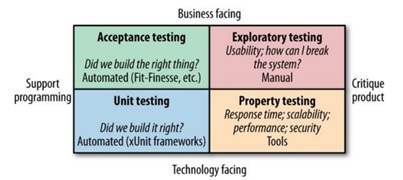
\includegraphics[width=1\textwidth]{test_types.jpg}
    \caption{Rodzaje testów. Źródło: \cite{newman2015}}
    \label{fig:test-types}
\end{figure}

Dwie kategorie znajdujące się na dole - \textit{unit testing} oraz \textit{property testing} - mają 
pomóc deweloperom utworzyć działający kod. Tego rodzaju testy mają na celu 
sprawdzenie, czy system nie jest obciążony usterkami związanymi z implementacją. 
Celem testów należących do dwóch kategorii znajdujących się na górze - \textit{acceptance 
testing} oraz \textit{exploratory testing} - jest pomoc w zrozumieniu jak dany system działa. 
Do tego rodzaju testów można zaliczyć m. in. szerokie testy obejmujące działanie dużej 
liczby mikroserwisów, sprawdzenie funkcjonalności systemu oraz tzw. \textit{user acceptance 
testing}, czyli testy przeprowadzone przez klienta, który zlecił budowę systemu.

\subsection{Testy jednostkowe}

Tego rodzaju testy sprawdzają poprawność pojedynczej metody w kodzie. Nie sprawdza się działania 
się całego mikroserwisu, a jedynie jego wyodrębioną część. Wszystkie parametry, które 
przyjmuje dana funkcja, są tworzone w trakcie testu. Testy jednostkowe są wykonywane 
w pierwszej fazie testów ze względu na szybkość ich wykonania. Ich celem jest wykrycie 
błędów związanych z daną technologią, nie zaś sprawdzenie, czy działanie systemu jest 
zgodne z oczekiwaniami klienta. Należy zapewnić dużą liczbę testów 
jednostkowych, ponieważ jest to najszybszy sposób zlokalizowania potencjalnych awarii.

Przykładem jest poniższy test:

\begin{lstlisting}
    [Test]
    public void MeasurementsTooHighIndicatorsTest()
    {
        // Arrange
        var currentMeasurement = 
        CreateMeasurementSentEvent();
        var policy = TestPoliciesDataService
            .CreateNewRoomPolicyDto(
                15, 80, 0.3f, 2, 20, 0.1f);

        // Run
        var result = 
        _policyEvaluator!
            .Evaluate(currentMeasurement, policy);
        
        // Assert
        Assert.AreEqual(
            result.TemperatureStatus, 
            EvaluatorResult.TooHigh);
        Assert.AreEqual(
            result.IlluminanceStatus, 
            EvaluatorResult.TooHigh);
        Assert.AreEqual(
            result.HumidityStatus, EvaluatorResult.TooHigh);
    }
\end{lstlisting}

Sprawdza on działanie logiki odpowiedzialnej za porównanie aktualnie panujących 
warunków w pomieszczeniu z warunkami oczekiwanymi. Test składa się z trzech części:

\begin{itemize} % lista nienumerowana
    \item Arrange - przygotowanie niezbędnych komponentów potrzebnych do przetestowania 
    fragmentu kodu
    \item Run - faktyczne uruchomienie testowanego kodu
    \item Assert - sprawdzenie otrzymanego wyniku z oczekiwanym rezultatem
\end{itemize}

\subsection{Testy integracyjne}

Testy integracyjne mają na celu sprawdzenie, czy poszczególne mikroserwisy będą 
w stanie się ze sobą skutecznie komunikować. Przykładem jest poniższy test:

\begin{lstlisting}
    [Test]
    public async Task 
    GetExpectedRoomConditionsAvailabilityTest()
    {
        var path = 
        $"policies-api/expected-room-conditions/1";
    
        var response = await _client.GetAsync(path);
    
        response.StatusCode.Should().Be(HttpStatusCode.OK);
    }    
\end{lstlisting}

Klient testowy korzysta z oferowanej przez testowany mikroserwis usługę poprzez 
wysłanie żądania http. W tym przypadku nie jest testowana logika zawarta w testowanym 
mikroserwisie, a jedynie odpowiedź, którą odsyła. Status odpowiedzi powinien oznaczać 
sukces, sygnalizowany przez kod 200 OK \cite{fielding1999}.

\subsection{Testy end-2-end}

Testy typu end-2-end mają za zadanie przetestować pewne biznesowe 
funkcjonalności, których realizacja może być obsługiwana przez wiele mikroserwisów. 
Dobrą praktyką jest utrzymywanie niewielkiej liczby tego typu testów, ponieważ 
obejmują one zakres działania całego systemu i przeprowadzenie każdego z nich zajmuje dużo 
czasu. Ponadto, w przypadku wystąpienia usterki ciężko jest wykryć miejsce, które 
było źródłem błędu.
Przykładem jest poniższy test, napisany w języku programowania Python:

\begin{lstlisting}
def measurement_triggers_policies_evaluation_result_event():
    new_measurement_test_helper = NewMeasurementTestHelper()

    new_measurement_test_helper
        .check_influxdb_is_available()

    new_measurement_test_helper
        .check_sensors_api_is_available()

    new_measurement_test_helper
        .send_new_measurement_to_rabbitmq()

    new_measurement_test_helper
    .check_message_sent_to_queue(
        new_measurement_test_helper
        .rabbitmq_configuration.vhost,
        consts.sensors_test_queue, 
        1)

    new_measurement_test_helper.
    check_message_sent_to_queue(
        new_measurement_test_helper
        .rabbitmq_configuration.vhost,
        consts.measurement_sent_event_test_queue, 
        1)

    new_measurement_test_helper.
    check_message_sent_to_queue(
        new_measurement_test_helper
        .rabbitmq_configuration.vhost,
        consts.policies_evaluation_result_event_test_queue, 
        1)
\end{lstlisting}

W tym teście sprawdza się odpowiedź całego systemu na otrzymanie nowego pomiaru 
z sensora. Jako skutek powinna zostać wygenerowana odpowiednia wiadomość z wynikiem 
przetworzenia pomiaru, która została wysłana na kolejkę wiadomości.

\subsection{Automatyzacja testów}

Ręczne uruchamianie każdego z testów pojedynczo może szybko stać się żmudnym zajęciem. 
Aby temu zaradzić, w ramach pracy inżynierskiej wykorzystano narzędzie do automatyzacji 
o nazwie Nuke \cite{nuke2022}. 
Za jego pomocą uruchomienie wszystkich testów sprowadza się do wykonania 
jednej komendy. 

Nuke pozwala na tworzenie własnych metod zwanych zamiarami (ang. \textit{target}), które automatyzują 
wykonywanie pewnych czynności. Każdy z zamiarów wykonuje określoną logikę. 
Dodatkowo, można tworzyć kompleksową strukturę, w której każdy z zamiarów jest zależny 
od tego, czy prawidłowo zostanie wykonany inny. Istnieje także możliwość 
dodania reguły wyzwalania poszczególnych zamiarów po wykonaniu innego. 
Przykładowo, metoda uruchamiająca test dla konkretnego projektu wygląda w sposób 
następujący:

\begin{lstlisting}
Target TestProject => _ => _
.DependsOn(CompileTestProject)
.Executes(() =>
{
    var solution = (this as IHaveSolution).Solution;
    var project = solution
        .AllProjects
        .Single(x => 
        x.Name == TestProjectNames[ProjectName]);
    DotNet($"test {project} --no-build -c {Configuration}");
});
\end{lstlisting}

Wykonuje ona metodę \textit{dotnet test}, uruchamianą dla konkretnego projektu. 
Wykonanie zamiaru zależy od pomyślnego wykonania innego, o nazwie \textit{CompileTestProject}.

\begin{lstlisting}
Target CompileTestProject => _ => _
.DependsOn(RestoreTestProject)
.Executes(() =>
{
    var solution = (this as IHaveSolution).Solution;
    var project = solution
        .AllProjects
        .Single(x => 
        x.Name == TestProjectNames[ProjectName]);
    DotNetBuild(s => s
        .EnsureNotNull(
            this as IHaveSolution, (_, o) => 
            s.SetProjectFile(project))
        .SetConfiguration(Configuration)
        .EnableNoRestore());
});
\end{lstlisting}

Metoda wykonuję komendę \textit{dotnet build}. Jest ona 
zależna od zamiaru \textit{RestoreTestProject}.

\begin{lstlisting}
Target RestoreTestProject => _ => _
.DependsOn(Clean)
.Requires(() => ProjectName)
.Executes(() =>
{
    var solution = (this as IHaveSolution).Solution;
    foreach (var proj in solution.AllProjects)
    {
        Logger.Info(proj.Name);
    }
    var project = solution
        .AllProjects
        .Single(x => 
        x.Name == TestProjectNames[ProjectName]);
    DotNetRestore(s => 
    s.EnsureNotNull(
        this as IHaveSolution, (_, o) => 
        s.SetProjectFile(project)));
});
\end{lstlisting}

Metoda wykonuje funkcję \textit{dotnet restore}. Jednym z 
warunków uruchomienia tego zamiaru jest konieczność podania nazwy projektu, wyrażona 
przez funkcję \textit{.Requires(() => ProjectName)}. Uruchomienie zamiaru jest zależne od poprawnego
wykonania innego, o nazwie \textit{Clean}.

\begin{lstlisting}
Target Clean => _ => _
.Executes(() =>
{
    SourceDirectory
    .GlobDirectories("**/bin", "**/obj")
    .ForEach(DeleteDirectory);
    EnsureCleanDirectory(ArtifactsDirectory);
});
\end{lstlisting}

Metoda czyści repozytorium z artefaktów. Nie jest zależna od żadnego innego zamiaru.
Wszystkie zamiary można uruchomić jednocześnie przy pomocy jednej metody:

\begin{lstlisting}
./build.sh TestProject --ProjectName facilities 
    --verbosity verbose
\end{lstlisting}
\newpage
\section{Pomiary}

W ramach tej pracy inżynierskiej przygotowano zestaw pomiarowy, który 
w regularnych odstępach czasu bada aktualną wartość temperatury oraz
natężenia światła. Zestaw został złożony z następujących elementów:

\begin{itemize} % lista nienumerowana
    \item Moduł WEMOS D1 Uno R3 ESP8266 WIFI
    \item Fotorezystor LDR GL5528
    \item Czujnik temperatury i wilgotności DHT11
    \item Rezystory 1 kOhm
\end{itemize}

Moduł WEMOS jest mikrokontrolerem oparty o kontroler ATmega328P. Posiada
11 portów wejścia-wyjścia pozwlających na dołączenie zewnętrznych 
urządzeń. Płytka została fabrycznie wyposażona w moduł wifi ESP8266. Za
jego pomocą mogą zostać wysłane pomiary.

Fotorezystor służy do pomiaru natężenia światła. Został wykonany 
z półprzewodników, które w temperaturze działania nie mają elektronów 
w paśmie przewodnictwa. Padające na półprzewodnik fotony o energii 
większej od przerwy energetycznej przemieszczają elektrony z pasma 
walencyjnego do pasma przewodnictwa, w wyniku którego powstają pary 
dziura-elektron. Zjawisko nazywane jest efektem fotoelektrycznym 
wewnętrznym.

Czujnik temperatury i wilgotności DHT11 bada aktualne wartości tych
dwóch parametrów. Mierzony zakres temperatury to -20\degree  - +60\degree C.
Jego rozdzielczość wynosi 0.1\degree C, a dokładność 2\degree C.

\subsection{Oprogramowanie mikrokontrolera}

Do rozwoju oprogramowania do mikrokontrolera WEMOSC wykorzystano narzędzie 
Arduino IDE, będące rozbudowanym edytorem pozwalającym na kompilację,
przesyłanie plików wykonywalnych na płytkę przy pomocy kabla USB oraz
debugowanie i podgląd logów produkowanych przez mikrokontroler w czasie 
rzeczywistym. Do utworzeniu kodu został wykorzystany język C.

Zadaniem mikrokontrolera było:

\begin{itemize} % lista nienumerowana
    \item Zebranie aktualnych pomiarów temperatury i natężenia światła
    \item przygotowanie wiadomości z uzyskanymi pomiarami
    \item wysłanie wiadomości przy pomocy protokołu MQTT przez moduł WIFI na 
    kolejkę brokera wiadomości RabbitMQ
\end{itemize}

Poniżej został przedstawiony przygotowany kod.

\begin{lstlisting}
    #include "rabbitmq_handler.h"

    #define WIFI_SSID "Tech_D0054234"
    #define WIFI_PASS "PASSWORD"
     
    void setup() {
      Serial.begin(115200);
      dht.begin();
      Serial.println();
     
      WiFi.mode(WIFI_STA);
      WiFi.begin(WIFI_SSID, WIFI_PASS);
     
      while (WiFi.status() != WL_CONNECTED)
      {
        delay(100);
      }
      
      client.setServer(RABBITMQ_BROKER, RABBITMQ_PORT);
      client.setCallback(callback);
    }
     
    void loop() {
      if ( !client.connected() ) {
        reconnect();
      }
      
      float temperature = readTemperature(&dht);
      int illuminance = analogRead(ILLUMINANCEPIN);
      publish_measurements(temperature, illuminance, false);
      
      delay(60000);
    
      client.loop();
    }
\end{lstlisting}

Każdy z programów wgrywanych na płytkę powinien zawierać dwie główne funkcje:

\begin{itemize}
    \item void setup() - wewnątrz metody definiowane są obiekty oraz zmienne 
    potrzebne przez cały czas działania mikrokontrolera
    \item void loop() - metoda wywoływana jako druga w kolejności po setup(),
    jest powtarzana przez resztę cyklu działania mikrokontrolera 
\end{itemize}

Na początku definiowana jest szyna, za pomocą której przesyłane są dane do 
modułu WIFI. Moduł wspiera prędkość transmisji na poziomie 115200 bitów na 
sekundę (ang. baud rate). Następnie tworzony jest klient, którego zadaniem
jest wysyłanie pomiarów na kolejkę brokera wiadomości. 

Wewnątrz metody loop() co 60 sekund zbierane są pomiary, po czym publikowane
na kolejkę. Pomiary wykonywane są przy użyciu poniższego kodu.

\begin{lstlisting}
    #include "DHT.h"

    #define DHTPIN 4
    #define DHTTYPE DHT11
    
    int ILLUMINANCEPIN = A0;
    
    DHT dht(DHTPIN, DHTTYPE);
    
    float readTemperature(DHT *dht){
      float t = dht->readTemperature();
     
      if (isnan(t))
      {
        Serial.println(
            "Error while reading current 
            temperature value");
      }
      
      return t;
    }
\end{lstlisting}

Główną rolę pełni obiekt dht, za pomocą którego można komunikować się
z czujnikiem. Zdefiniowany jest typ czujnika przy użyciu makra DHTTYPE.
Numer pinu, do którego został wpięty kabel łączący płytkę z czujnikiem,
został oznaczony pzy użyciu makra DHTPIN. Pomiar temperatury odbywa się
przez wywołanie funkcji readTemperature(). 

Pomiar z fotorezystora można odczytać przy użyciu komendy:  

\begin{lstlisting}
    analogRead(ILLUMINANCEPIN)
\end{lstlisting}

gdzie ILLUMINANCEPIN oznacza numer pinu, do 
którego wpięty jest kabel łączący płytkę z fotorezystorem.

Poniższy kod zawiera szczegóły implementacyjne dotyczące 
wysyłania wiadomości na kolejkę.



Warto wyjaśnić wartości zmiennych związanych z brokerem wiadomości:
\begin{lstlisting}
    const char* RABBITMQ_BROKER = "192.168.0.12";
    int        RABBITMQ_PORT     = 1883;
    const char* RABBITMQ_TOPIC  = "room_measurements";
    const char* RABBITMQ_SUBSCRIPTION  
    = "request_measurement";
    const char* RABBITMQ_USER = "guest";
    const char* RABBITMQ_PASSWORD = "guest";
    const char* RABBITMQ_SENSOR_ID = "968376";
\end{lstlisting}

\begin{itemize}
    \item RABBITMQ\_BROKER: adres IP serwera, na którym uruchomiony jest broker wiadomości
    \item RABBITMQ\_PORT: numer portu serwera, na którym nasłuchuje broker
    \item RABBITMQ\_TOPIC: temat, na który wysyłane są wiadomości z mikrokontrolera
    na kolejkę
    \item RABBITMQ\_SUBSCRIPTION: temat, na który nasłuchuje mikrokontroler
    \item RABBITMQ\_USER: nazwa użytkownika, za pomocą którego płytka jest uwierzytelniana
    \item RABBITMQ\_PASSWORD: hasło dla wykorzystywanego użytkownika
\end{itemize}

Wiadomość do brokera jest wysyłana w metodzie send\_measurements:

\begin{lstlisting}
    void send_measurements(
        float temperature, int illuminance){
      char temperatureChar[64];
      int ret = snprintf(
          temperatureChar, sizeof temperatureChar, 
          "%f", temperature);
      if (ret < 0) {
          return;
      }
      if (ret >= sizeof temperatureChar) {
           return;
      }
      char illuminanceChar[64];
      ret = snprintf(
          illuminanceChar, sizeof illuminanceChar, 
          "%d", illuminance);
      if (ret < 0) {
          return;
      }
      if (ret >= sizeof illuminanceChar) {
           return;
      }
    
      char* measurement = (char*)malloc(256+1+3); 
      //4*64 + 3 semicolons + EOF
      strcpy(measurement, temperatureChar);
      strcat(measurement, ";");
      strcat(measurement, illuminanceChar);
      strcat(measurement, ";");
      strcat(measurement, RABBITMQ_SENSOR_ID);
    
      time_t t = time(NULL);
      struct tm tm = *localtime(&t);
    
      client.publish(RABBITMQ_TOPIC, measurement);
    
      free(measurement);
    }
\end{lstlisting}

Mikrokontroler nasłuchuje na wiadomości o temacie \\RABBITMQ\_SUBSCRIPTION:

\begin{lstlisting}
    void callback(
        char* topic, byte* payload, unsigned int length) {
      char* sensorId = (char*)payload;
    
      String messageTemp;
      
      for (int i = 0; i < length; i++) {
        Serial.print((char)payload[i]);
        messageTemp += (char)payload[i];
      }
    
      if(strcmp(topic, RABBITMQ_SUBSCRIPTION) 
      == 0 && strcmp(sensorId, RABBITMQ_SENSOR_ID)){
        float temperature = readTemperature(&dht);
        int illuminance = analogRead(ILLUMINANCEPIN);
        publish_measurements(
            temperature, humidity, illuminance, true);
      }
    }
\end{lstlisting}
\newpage
\section{Automatyzacja}
Sekcja przedstawia narzędzia wykorzystane do automatyzacji procesu rozwoju i wdrażania
systemu. Podrozdział 9.1 opisuje zasady działania platformy Docker oraz sposób jej 
wykorzystania w pracy. Podrozdziały 9.2 - 9.3 przybliżają metodyki ciągłej
integracji oraz ciągłego dostarczania, bezpośrednio powiązanymi z automatyzacją
rozwiązania. W podrozdziale 9.4 opisano zasady działania oraz sposób wykorzystania
narzędzia do orkiestracji systemu Kubernetes.

Pełna automatyzacja regularnie wykonywanych zadań, pozwalająca znacznie przyspieszyć 
wdrażanie całości systemu, była jednym z najważniejszych zagadnień poruszonych w 
trakcie tworzenia pracy. Prawidłowe podejście do wdrażania aplikacji znacząco wpływa 
na szybkość, z jaką zmiany wprowadzone lokalnie mogą zostać wykorzystane w 
produkcyjnej wersji systemu. 

\subsection{Docker}
Sekcja zawiera opis zasad działania oraz sposób wykorzystania platformy Docker.
Podrozdział 9.1.1 przybliża sposób komunikacji kontenerów ze sobą oraz ze
światem zewnętrznym. 

Docker jest otwartą platformą do rozwoju oraz wdrażania aplikacji. Pozwala oddzielić aplikacje od
dostępnej na danym serwerze infrastruktury, co pozwala przyspieszyć proces dostarczania najnowszych
wersji systemu. 

Platforma zapewnia możliwość spakowania i uruchomienia aplikacji w odizolowanym środowisku
zwanym kontenerem. Izolacja powoduje, że możliwe jest bezpieczne uruchomienie wielu kontenerów na tym
samym hoście. Platforma pozwala zarządzać infrastrukturą potrzebną do uruchomienia kontenera, dzięki
czemu eliminowany jest problem instalacji wszystkich wymaganych zależności na każdym serwerze z osobna.

Docker wykorzystuje architekturę typu klient-serwer. Klient komunikuje się z tzw. \textit{docker daemon}, którego
zadaniem jest budowanie, uruchamianie oraz dystrybuowanie kontenerów. 

W celu utworzenia kontenerów należy w pierwszej kolejności utworzyć ich obraz, który jest szablonem
zawierającym instrukcje dotyczące jego budowy. Szablony są przechowywane w plikach o nazwie \textit{Dockerfile}.
Każda instrukcja tworzy jedną warstwę obrazu. Mechanizm ten jest szczególnie przydatny, gdy szablony są
regularnie rozwijane o nowe instrukcje. Wtedy, przy ponownym budowaniu obrazu, tylko warstwy, które
uległy zmianie są odświeżane. Pozwala to znacznie przyspieszyć proces budowania obrazów.

Kontener jest instancją obrazu, którą można uruchomić. Działa on tak długo, dopóki nie zostanie
zakończony proces główny.

Przykładowy szablon, który przedstawia obraz ADS, został przedstawiony poniżej:

\begin{lstlisting}
FROM mcr.microsoft.com/dotnet/aspnet:5.0 AS base
WORKDIR /app
EXPOSE 80
EXPOSE 443

FROM mcr.microsoft.com/dotnet/sdk:5.0 AS build
WORKDIR /app
COPY [".", "."]

RUN dotnet restore 
    ./DagAir_Addresses/DagAir.Addresses
    /DagAir.Addresses.csproj
RUN dotnet build 
    ./DagAir_Addresses/DagAir.Addresses
    /DagAir.Addresses.csproj 
    --no-restore
RUN dotnet publish 
    ./DagAir_Addresses/DagAir.Addresses
    /DagAir.Addresses.csproj 
    -c Release -o /app/publish

FROM base AS final
WORKDIR /app
COPY --from=build /app/publish .
ENTRYPOINT ["dotnet", "DagAir.Addresses.dll"]
\end{lstlisting}

Pierwszym etapem jest utworzenie obrazu pośredniego o nazwie base. Oparty on jest na obrazie 
aspnet:5.0 dostępnym publicznie na platformie dockerhub \cite{aspnet2022}.
Na tym etapie deklarowane są
numery portów, na których aplikacja powinna nasłuchiwać na przychodzące żądania.

Drugim etapem jest utworzenie obrazu pośredniego, opartego o obraz sdk:5.0, który także jest dostępny publicznie
na platformie dockerhub \cite{dotnetsdk2022}. Na tym etapie kopiowane
są wszystkie zależności, których wymaga aplikacja, by mogła zostać prawidłowo uruchomiona.
Za pomocą komend oferowanych przez dotnet CLI publikowana jest gotowa do wdrożenia wersja aplikacji.

W ostatnim etapie kopiowana jest wersja aplikacji przygotowana w ramach etapu drugiego, po czym
następuje uruchomienie procesu za pomocą komendy:

\begin{lstlisting}
    dotnet DagAir.Addresses.dll
\end{lstlisting}

Podział na poszczególne etapy wynika z różnych rozmiarów wykorzystywanych obrazów. Możliwe byłoby
utworzenie obrazu aplikacji na podstawie obrazu sdk:5.0. Jednak jego rozmiar to ok. 630 MB, podczas
gdy rozmiar obrazu aspnet:5.0 to ok. 205 MB. Dzięki temu prostemu zabiegowi można oszczędzić 
znaczną część zasobów obliczeniowych. 

Dzięki szablonom można tworzyć obrazy poszczególnych serwisów. Jednak uruchamianie każdego z nich
pojedynczo byłoby kosztownym czasowo zajęciem. Rozwiązaniem tego problemu jest wykorzystanie narzędzia
\textit{docker-compose}, które umożliwia uruchamianie wielu kontenerów za pomocą jednej komendy. W tym celu
należy przygotować szablon zawierający instrukcje uruchomienia każdego z utworzonych na wcześniejszym
etapie obrazów. Szablon jest przechowywany w pliku o nazwie \textit{docker-compose.yml}.

Przykładowy szablon został przedstawiony poniżej:

\begin{lstlisting}
    version: "3.9"
    services:
      addresses_api:
        build:
          target: final
          context: ./src
          dockerfile: ./DagAir_Addresses/Dockerfile
        environment:
          - ASPNETCORE_ENVIRONMENT=Docker
          - ConnectionKeys__DagAir.Addresses=
                ${ADDRESSES_CONNECTIONKEYS}
        ports:
          - "8094:80"
        networks:
          - dagair_network
        restart: always

    networks:
    dagair_network:
\end{lstlisting}

W szablonie został przedstawiony proces uruchomienia ADS. Zdefiniowano:

\begin{itemize}
    \item Szablon obrazu, z którego należy skorzystać
    \item Zmienne środowiskowe potrzebne do uruchomienia aplikacji w środowisku dockerowym
    \item Port, na którym ma nasłuchiwać aplikacja. Występuje tutaj mapowanie między portem 
    serwera, na którym będzie uruchomiony kontener, a portem w kontenerze. Dzięki mapowaniu
    aplikacja będzie dostępna na serwerze pod adresem:

    \begin{lstlisting}
        http://localhost:8094/
    \end{lstlisting}
    \item Wirtualna sieć, do którego ma zostać dołączony kontener w środowisku dockerowym
    \item Polityka ponownego uruchamiania. Flaga \textit{always} oznacza, że w przypadku zatrzymania pracy
    instancji kontenera, zostanie ona usunięta, a na jej miejsce zostanie uruchomiona nowa
\end{itemize}

\subsubsection{Łączność sieciowa w środowisku skonteneryzowanym}
\label{subsubection:lacznosc-sieciowa-docker}
W celu zapewnienia izolacji między procesami różnych kontenerów wykorzystuje się
przestrzenie nazw (ang. \textit{namespace}). Jest to funkcjonalność polegająca na podziale zasobów w taki sposób, aby
każdy zestaw procesów korzystał z innej, wydzielonej części. Przestrzeni nazw przypisuje się dedykowany
interfejs, za pomocą którego może komunikować się z innymi przestrzeniami. Łączność między kontenerami
jest osiągana poprzez połączenie utworzonych interfejsów za pomocą mostu (ang. \textit{bridge}).
Pełni on rolę tzw. \textit{switch'a} odpowiedzialnego za przesyłanie pakietów między przestrzeniami nazw
w oparciu o protokół ARP lub IP. Do mostu dołączony jest także interfejs pozwalający na komunikację
z procesami uruchomionymi na oddzielnych maszynach.

Rysunek \ref{fig:container-networking} przedstawia podział zasobów na przestrzenie nazw.

\begin{figure}[h]
  \centering
  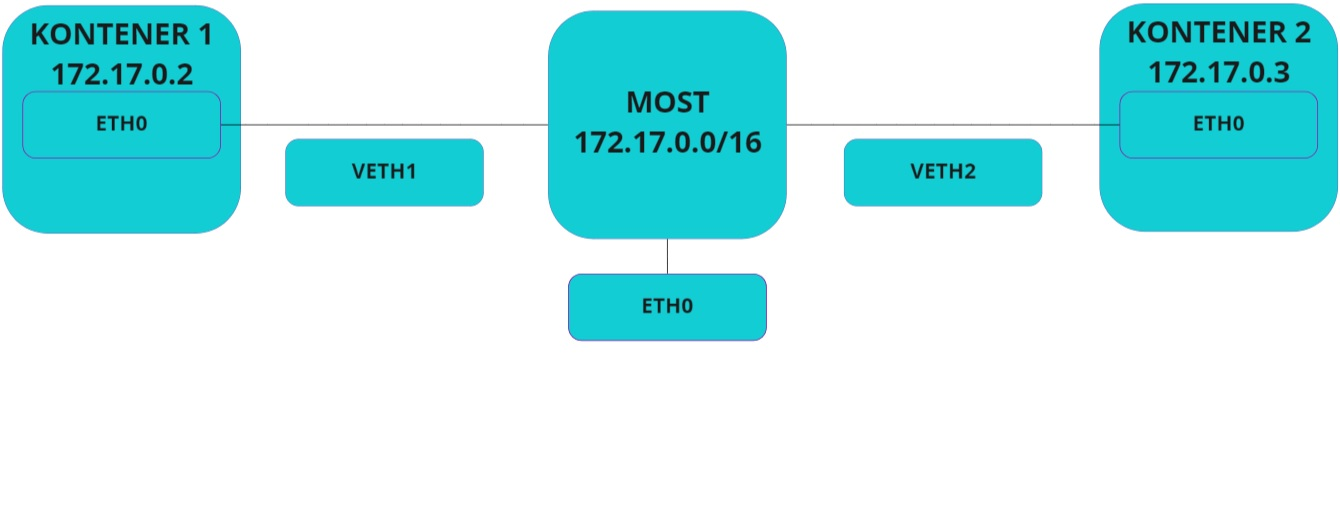
\includegraphics[width=1\textwidth]{container_networking.jpg}
  \caption{Łączność sieciowa w środowisku skonteneryzowanym. Opracowanie własne}
  \label{fig:container-networking}
\end{figure}

Platforma docker domyślnie tworzy most należący do podsieci 172.17.0.0/16.

Każdy kontener może uruchamiać procesy, które będą nasłuchiwać żądań na ustalonych portach.
Przestrzenie nazw posiadają oddzielne zestawy portów, dzięki czemu w każdej z nich może
zostać uruchomiony proces nasłuchujący przykładowo na porcie 80. Mapowanie portów w środowisku
kontenerów polega na skojarzeniu portów udostępnianych przez maszynę, na której uruchomione sobą
kontenery, z portami udostępnianymi przez przestrzenie nazw. Poniższy fragment przedstawia 
mapowanie między portem 80 udostępnianym przez przestrzeń nazw, w której uruchomiono mikrousługę ADS, 
a portem 8094 udostępnianym przez hosta:

\begin{lstlisting}
  ports:
      - "8094:80"
\end{lstlisting}

Dzięki temu usługi oferowane przez ten moduł danych są dostępne
pod adresem \textit{http://localhost:8094}.

\subsection{Ciągła integracja}

Podstawowym wymaganiem, które należy spełnić przy tworzeniu rozbudowanych systemów 
informatycznych, jest przechowywanie rozwijanego oprogramowania przy pomocy wybranego 
narzędzia kontroli wersji, takiego jak Git \cite{git2022}. Dane są zapisywane w folderze zwanym 
repozytorium. Zadaniem takiego narzędzia jest śledzenie wprowadzonych zmian 
oprogramowania i zapisywanie ich w historii repozytorium. Zapewnia to wiele 
korzyści, z których najważniejsze to:

\begin{itemize} % lista nienumerowana
    \item Podgląd zmian wprowadzonych przez każdego dewelopera
    \item Możliwość powrotu do poprzedniej wersji w przypadku, gdy wprowadzone zmiany 
    były przyczyną błędów w działaniu systemu
\end{itemize}

Głównym celem ciągłej integracji (ang. \textit{continuous integration}) jest regularne włączanie 
bieżących zmian w kodzie do głównego repozytorium i każdorazowa weryfikacja 
wprowadzonych zmian poprzez utworzenie nowego zbioru plików wykonywalnych 
i przeprowadzenie na nich testów jednostkowych. Zaletą tego podejścia jest fakt, że 
po wysłaniu przez programistę zmian do repozytorium głównego, reszta czynności 
wykonywana jest automatycznie przez serwer ciągłej integracji, bez ingerencji 
człowieka. Dodatkowo programista otrzymuje szybką odpowiedź zwrotną w razie 
wystąpienia błędów.
Aby wykorzystać potencjał ciągłej integracji, należy zwrócić uwagę na następujące 
punkty: 

\begin{itemize} % lista nienumerowana
    \item Częste i regularne wysyłanie kodu do głównego repozytorium w celu weryfikacji 
    integracji nowych zmian z resztą kodu, przynajmniej raz dziennie 
    \item Zapewnienie testów jednostkowych sprawdzających poprawność zachowania systemu. 
    Może się zdarzyć, że wprowadzone zmiany będą zgodne pod względem 
    składni, jednak nie oznacza to, że serwis będzie prawidłowo spełniał swoje 
    funkcje 
    \item Nadanie wysokiego priorytetu naprawieniu kodu, który nie integruje się z 
    dotychczasowym kodem w repozytorium. Odkładanie poprawy na później może spowodować 
    spiętrzenie się kolejnych błędów, co w konsekwencji bardziej spowolni wdrażanie 
    nowych funkcji
\end{itemize}

W trakcie tworzenia pracy wykorzystano platformę do ciągłej integracji i wdrażania 
o nazwie Github Actions. Pozwala ona na automatyzację tworzenia nowych wersji 
oprogramowania, testowania oraz wdrażania. Kolejne powtórzenia przepływów pracy 
(ang. \textit{workflow}) są wykonywane na maszynach wirtualnych oferowanych przez 
GitHub, zwanych pracownikami (ang. \textit{worker}). W zależności od potrzeby na maszynach 
zainstalowany jest odpowiedni system operacyjny spośród sytrybucji 
linux-owych, Windowsa oraz macOS.

\textit{GitHub Action} jest przepływem pracy, który może zostać wywołany zawsze wtedy, gdy 
zostanie zarejestrowane nowe zdarzenie dotyczące wykorzystywanego repozytorium. 
Przykładem zdarzenia jest wprowadzenie nowych zmian do repozytorium lub utworzenie 
żądania typu \textit{pull request}. \textit{GitHub Action} składa się z jednej lub większej liczby 
zadań (ang. \textit{job}), które mogą zostać wykonane jedno po drugim lub równolegle. Z kolei 
każde zadanie składa się z jednego lub większej liczby kroków (ang. \textit{step}), z których 
każde może wykonać własnoręcznie utworzony skrypt lub akcję (ang. \textit{action}), będącą 
rozszerzeniem umożliwiającym uproszczenie całego przepływu pracy.

Przykładowy przepływ pracy utworzony na potrzeby projektu wykonuje następujące zadania:

\begin{itemize} % lista nienumerowana
    \item Wybiera odpowiednią gałąź z repozytorium, na której zostały wprowadzone 
    nowe zmiany
    \item Instaluje wymagane oprogramowanie niezbędne do wykonania wszystkich 
    pozostałych zadań, takie jak środowisko .NET 5.0
    \item Uruchamia testy jednostkowe i integracyjne
    \item Tworzy nową wersję obrazu sprawdzonego mikroserwisu
    \item Wypycha obraz do rejestru kontenerów
\end{itemize}

Warto szczegółowo prześledzić poszczególne kroki danego przepływu.

\begin{lstlisting}
jobs:
  docker-build-and-push:
    runs-on: ubuntu-latest
    steps:
    - name: Checkout
      uses: actions/checkout@v2
      with:
        fetch-depth: 0
\end{lstlisting}

Powyższy wyciąg deklaruje nowe zadanie oraz pierwszy z kroków, który wybierze 
odpowiędnią gałąź z repozytorium. Parametr runs-on wskazuje jaki rodzaj systemu 
operacyjnego powinien zostać wykorzystany.

\begin{lstlisting}
on:
  workflow_dispatch: # allows to trigger workflow on demand
  push:
    branches: 
      - main
      - develop
    paths:
      - src/DagAir_Facilities/**
\end{lstlisting}

GitHub Actions oferuje rozbudowany system do określania warunków, które muszą być 
spełnione, aby uruchomić przepływ pracy. Powyższy wyciąg przedstawia fragment, który 
określa, że przepływ ma być uruchomiony gdy:

\begin{itemize} % lista nienumerowana
    \item Użytkownik manualnie uruchomi przepływ za pomocą interfejsu graficznego
    \item Zostaną wprowadzone nowe zmiany na gałęzi main lub develop oraz zmiany będą 
    się znajdować w katalogu \textit{src/DagAir\_Facilities/}
\end{itemize}

\begin{lstlisting}
- name: Build & Test
    shell: bash
    run: ./build.sh TestProject 
        --ProjectName facilities --verbosity verbose
\end{lstlisting}

Powyższy krok wykonuje skrypt uruchamiający testy jednostkowe oraz integracyjne.

\begin{lstlisting}
- name: Set image names & main tags
run: |
  appImageName="${{ env.
    CONTAINER_REGISTRY }}/${{ env.SERVICE_NAME }}"
  migrationsApplierImageName=
    "${{ env.CONTAINER_REGISTRY }}/${{ env.
    MIGRATIONS_APPLIER_NAME }}"
  echo "APP_IMAGE_NAME=$appImageName" >> $GITHUB_ENV
  echo "MIGRATIONS_APPLIER_IMAGE_NAME
    =$migrationsApplierImageName" 
    >> $GITHUB_ENV

  version="${{ steps.gitversion.outputs
    .nugetVersionV2 }}-${{ steps.gitversion
    .outputs.shortSha }}"

  if [ ${{ steps.gitversion.outputs
    .commitsSinceVersionSource }} -gt 0 ]; then
  version="${{ steps.gitversion.outputs
    .escapedBranchName }}-$version"
  fi

  echo "APP_IMAGE_TAG=${appImageName}:$version" 
    >> $GITHUB_ENV
  echo "MIGRATIONS_APPLIER_IMAGE_TAG=
  ${migrationsApplierImageName}:$version" \
  >> $GITHUB_ENV
\end{lstlisting}

Powyższy krok generuje nazwę oraz tag nowego obrazu testowanego mikroserwisu. Na nazwę 
obrazu składa się nazwa repozytorium obrazów oraz nazwa mikroserwisu. Numer wersji 
obrazu za każdym razem powinien być unikalny, ponadto powinien wskazywać, która z 
wersji obrazu jest najnowsza. Wobec tego na wersję składa się nazwa gałęzi 
repozytorium, nazwa utworzonej paczki Nuget-owej oraz krótki unikalny numer przypisany 
do migawki (ang. \textit{commit}), która spowodowała uruchomienie przepływu.

\begin{lstlisting}
- name: Docker login
  uses: docker/login-action@v1
  with:
    registry: ${{ env.CONTAINER_REGISTRY }}
    username: ${{ secrets.AZURE_CR_USERNAME }}
    password: ${{ secrets.AZURE_CR_PASSWORD }}

- name: Docker push images
  run: |
    docker push ${{ env.APP_IMAGE_NAME }} --all-tags
    docker push ${{ env.MIGRATIONS_APPLIER_IMAGE_NAME }} 
        --all-tags
\end{lstlisting}

Na samym końcu gotowy obraz zostaje wypchnięty do repozytorium obrazów. W tym celu 
używana jest komenda \textit{docker push}. Aby zakończyła się pomyślnie, należało 
w poprzednim kroku zalogować się do repozytorium, wykorzystując nazwę repozytorium obrazów oraz 
danych uwierzytelniających, przechowywanych w bezpieczny sposób za pomocą Github 
Secrets.

\subsection{Ciągłe dostarczanie}

W trakcie prac nad systemem wykorzystano metodykę ciągłego dostarczania, która polega na tym, że kod 
przechodzi przez kolejne fazy testowania, gdzie za każdym razem jest weryfikowana jego poprawność pod 
względem prawidłowego funkcjonowania. 

Na początku przeprowadzane są szybkie testy jednostkowe sprawdzające punktowo poprawność 
poszczególnych funkcji. Jeśli zostaną wykonane pomyślnie, przechodzi się do następnej fazy 
testowania uwzględniające wolniejsze testy, które sprawdzają zachowanie wielu serwisów między 
sobą. Po upewnieniu się, że ta faza została wykonana pomyślnie, system jest weryfikowany przez 
klienta, który zlecał jego wykonanie (tzw. \textit{user acceptance testing}). Jeśli funkcjonalność zgadza się z 
oczekiwaniami klienta, całość jest jeszcze testowana pod kątem wydajności, po czym zostaje 
wdrożona na etap produkcyjny.

Zgodnie z założeniami metodyki, programiści powinni otrzymywać
wiadomości zwrotne dotyczące statusu kolejnych wersji 
oprogramowania w kolejnych fazach testowania. Wprowadzenie takiego potoku potrafi znacznie
poprawić ocenę jakości kodu, ponadto skrócić czas między wdrożeniem kolejnych wersji systemu.

\subsection{Kubernetes}
Sekcja opisuje zasady działania oraz sposób wykorzystania narzędzia Kubernetes.
Podrozdziały 9.4.1 - 9.4.2 przedstawiają poszczególne komponenty, z których
składa się narzędzie. Podrozdział 9.4.3 przybliża sposób komunikacji
kontenerów znajdujących się w klastrze ze sobą oraz ze światem zewnętrznym.

Kubernetes jest platformą do orkiestracji kontenerów automatyzującą procesy manualne 
związane z wdrażaniem, zarządzaniem oraz skalowaniem skonteneryzowanych aplikacji. 
Jest to oprogramowanie typu open-source, początkowo rozwijane przez firmę Google
\cite{kubernetes2022}.

W przeszłości, organizacje uruchamiały aplikacje na fizycznych serwerach. W momencie 
gdy wiele aplikacji działało w ramach jednego serwera, dochodziło do 
sytuacji, w których jedna z nich zajmowała większość zasobów, przez co inne 
nie działały optymalnie. Jednym z rozwiązań było uruchomienie każdej 
z aplikacji na innym fizycznym serwerze. Jednak w takim wypadku konsekwencjami były 
wysokie koszty utrzymania infrastruktury. Innym możliwym rozwiązaniem było wprowadzenie 
wirtualizacji, które przyczyniło się do bardziej zrównoważonego zarządzania zasobami. 
Efektem ubocznym było jednak wprowadzanie dużego nakładu zasobów potrzebnych na 
uruchomienie samej maszyny wirtualnej, ponieważ każda z maszyn instalowała na początku 
własny system operacyjny.

Najlepszym obecnie rozwiązaniem jest wykorzystanie kontenerów. Zawierają zestaw 
podobnych cech do maszyn wirtualnych z tą różnicą, że nie wymagają osobnego systemu 
operacyjnego. Każdy z kontenerów może współdzielić jeden system operacyjny z 
innymi, co znacznie obniża wymagania dotyczące zasobów. Podobnie do maszyn 
wirtualnych posiadają własny system plików, zasoby obliczeniowe, pamięć. Jednak nie 
zależą od infrastruktury, na której są uruchamiane, co czyni je przenośnymi wśród 
różnych dystrybucji danego systemu.

Kontenery stały się popularne ze względu na szereg zalet:

\begin{itemize} % lista nienumerowana
    \item Utworzenie obrazów następuje szybciej w porównaniu do maszyn wirtualnych
    \item Obrazy zostają utworzone na etapie budowania nowej wersji systemu zamiast na etapie wdrażania
    \item Niezależnie od środowiska działają w dokładnie ten sam sposób
    \item Mogą być uruchomione praktycznie na każdym systemie i dystrybucji
    \item Cechują się wysoką efektywnością wykorzystania zasobów
\end{itemize}

Rysunek \ref{fig:deployment-types}. przedstawia różnice między uruchomieniem aplikacji w sposób 
tradycyjny, przy użyciu maszyn wirtualnych oraz kontenerów.

\begin{figure}[h]
    \centering
    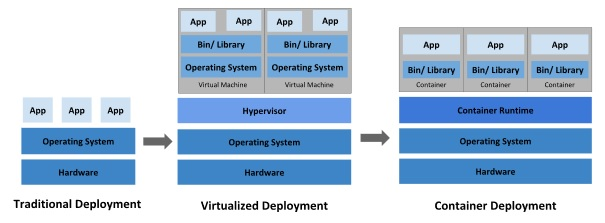
\includegraphics[width=1\textwidth]{deployment_types.jpg}
    \caption{Porównanie różnych metod uruchamiania aplikacji. Źródło: \cite{kubernetes2022}}
    \label{fig:deployment-types}
\end{figure}

Zalety Kubernetesa to przede wszystkim:

\begin{itemize} % lista nienumerowana
    \item Orkiestracja kontenerów między różnymi serwerami
    \item Efektywniejsze wykorzystanie zasobów
    \item Łatwe skalowanie skonteneryzowanych aplikacji 
    \item Zarządzanie serwisami w sposób deklaratywny
    \item Kontrola stanu aplikacji, automatyczne restartowanie kontenerów, 
    autoskalowanie
\end{itemize}

Zbiór hostów wykorzystywanych do uruchomienia na nich systemu zwany jest klastrem. Na 
każdym z hostów, zwanych węzłami, można uruchomić instancje gotowych obrazów. Każdy 
z klastrów posiada przynajmniej jeden węzeł.

Cyklem życiowym każdego kontenera zarządza płaszczyzna sterowania (ang. \textit{control 
plane}), która wystawia API oraz interfejsy umożliwiające ich wdrażanie i zarządzanie. 
Komponenty płaszczyzny mogą być uruchomione na każdej maszynie w klastrze, chociaż 
zazwyczaj określa się jedną maszynę, tzw. gospodarza (ang. \textit{master}), na której znajdują się 
wszystkie komponenty.

\subsubsection{Komponenty płaszczyzny sterowania}

W tabeli \ref{tab:komponenty-sterowania} zostały opisane komponenty składające się na całość płaszczyzny 
sterowania.
\newpage

\begin{xltabular}{1\textwidth} { 
  | >{\raggedright\arraybackslash}c 
  | >{\raggedright\arraybackslash}X | }
  \caption{Komponenty płaszczyzny sterowania} \label{tab:komponenty-sterowania}\\
  \hline
 Nazwa komoponentu & Opis \\
 \hline
 Kube-apiserver & Interfejs pozwalający na interakcję z płaszczyzną sterowania. 
 Weryfikuje i konfiguruje dane dla obiektów takich jak serwisy czy kontrolery 
 replikacji \\
 \hline
 Etcd & Spójny i wysoce dostępny magazyn par klucz-wartość używany przez Kubernetesa 
 jako miejsce do przechowywania wszystkich danych ważnych z punktu widzenia klastra.  \\
 \hline
 Kube-scheduler & Regularnie sprawdza czy został utworzony nowy zestaw 
 kontenerów, któremu nie został jeszcze przypisany węzeł. W takim przypadku wybiera 
 on maszynę, na której kontenery mają być uruchomione. Przy wyborze pod uwagę brane są 
 takie czynniki jak wymagane zasoby, ograniczenia sprzętowe lub programowe \\
 \hline
 Kube-controller-manager & Komponent odpowiedzialny za uruchamianie kontrolerów, które 
 monitorują oraz zmieniają stan klastra korzystając z API serwera \\
 \hline
 Cloud-controller-manager & Element, który wbudowuje logikę związaną z konkretną 
 chmurą, w której tworzone są klastry. Pozwala połączyć dany klaster z API dostawcy 
 chmury oraz oddziela komponenty, które oddziałują z chmurą od komponentów, które 
 oddziałują tylko z klastrem. Jest to komponent, który występuje tylko w przypadku 
 stawiania kontenerów w chmurze. Jeśli Kubernetes działa np. w prywatnym środowisku 
 na jednym komputerze, wtedy klaster nie posiada tego elementu \\
 \hline
\end{xltabular}

Istnieje kilka rodzajów kontrolerów:

\begin{itemize}
    \item Kontroler węzłów (ang. \textit{node controller}) - odpowiedzialny za wykrycie oraz 
    odpowiednią reakcję w przypadku, gdy jeden z węzłów ulega awarii lub staje się 
    niedostępny
    \item Kontroler prac (ang. \textit{job controller}) - nasłuchuje na pojawienie się obiektów 
    pracy (job objects) reprezentujących zadania, a następnie tworzy zbiór (pod) który 
    te zadania wykona
    \item Kontroler punktów końcowych - zarządza obiektami punktów końcowych (serwisy 
    oraz zbiory (ang. \textit{pods}))
    \item Kontroler kont oraz tokenów - tworzy domyślne konta oraz tokeny dostępu do 
    API dla nowych przestrzeni nazw
\end{itemize}

\subsubsection{Komponenty węzła}

W tabeli \ref{tab:komponenty-wezla} opisano komponenty, które działają na każdym węźle w Kubernetesie.

\begin{xltabular}{1\textwidth} { 
  | >{\raggedright\arraybackslash}c 
  | >{\raggedright\arraybackslash}X | }
  \caption{Komponenty węzła} \label{tab:komponenty-wezla}\\
  \hline
 Nazwa komponentu & Opis \\
 \hline
 Kubelet & Agent, którego rolą jest upewnienie się, że kontenery są uruchomione 
 w zbiorze (pods). Przyjmuje zestaw specyfikacji zbiorów i zapewnia, że wszystkie 
 kontenery podane w specyfikacji działają i są sprawne. Kubelet nie zarządza 
 kontenerami, które nie zostały utworzone przez Kubernetesa. \\
 \hline
 Kube-proxy & Proxy sieciowe, które implementuje część serwisu pozwalającego wystawić 
 aplikację do świata zewnętrznego. Jego zadaniem jest utrzymanie reguł sieciowych 
 w zarządzanych węzłach. Te reguły pozwalają na komunikację między różnymi zbiorami 
 wewnątrz lub na zewnątrz klastra.  \\
 \hline
 Container runtime & Oprogramowanie odpowiedzialne za uruchamianie kontenerów. 
 Kubernetes wspiera wiele możliwych runtime-ów, m. in. Docker, containerd, CRI-O. \\
 \hline
 Pod & Grupa złożona z jednego lub większej liczby kontenerów, wdrożona na tym samym 
 węźle. Wszystkie kontenery z grupy współdzielą adres IP oraz przydzielone zasoby. \\
 \hline
 Replication controller & Narzędzie do kontroli liczby kopii danego poda, które powinny 
 być w danej chwili uruchomione \\
 \hline
\end{xltabular}

Płaszczyzna sterowania przyjmuje komendy od administratora klastra, po czym przekazuje 
je do podległych serwerów. Komendy przyjmowane są za pomocą interfejsu 
konsolowego, zwanego \textit{kubectl}. Dobrą praktyką jest utworzenie plików deklarujących 
pożądany stan, w jakim powinien znajdować się klaster. Przykładowa deklaracja znajduje 
się poniżej.

\begin{lstlisting}
apiVersion: apps/v1
kind: Deployment
metadata:
  name: web-admin-app
  labels:
    app: web-admin-app
    tier: backend
spec:
  replicas: 2
  selector:
    matchLabels:
      app: admin-application-service
  template:
    metadata:
      labels:
        app: admin-application-service
        tier: backend
    spec:
      containers:
      - name: admin-application-service
        image: admin-application-service:develop-latest
        env:
        - name: ASPNETCORE_ENVIRONMENT
          value: "Kubernetes"
        imagePullPolicy: Always
        ports:
        - containerPort: 80
\end{lstlisting}

Jest to deklaracja typu \textit{Deployment}, która powinna zawierać następujące parametry:

\begin{itemize} % lista nienumerowana
    \item Wersja wykorzystywanego API
    \item Typ deklaracji
    \item Nazwa deklaracji
    \item Specyfikacja przedstawiająca pożądany stan, w jakim powinien znajdować się 
    klaster. W tym przypadku deklaruje się, że w klastrze powinny działać dwie 
    instancje obrazu mikrousługi aplikacyjnej dla administratorów, które powinny 
    nasłuchiwać na żądania na porcie 80
\end{itemize}

Komenda \textit{kubectl apply -f deployment.yml} umożliwia zaaplikowanie deklaracji.

Płaszczyzna sterowania jest odpowiedzialna za to, by stan klastra odpowiadał 
deklaracji. W konsekwencji zostaną utworzone dwa osobne pody, z których każdy otrzyma 
unikalny prywatny adres IP wewnątrz klastra. Od tej pory do każdej instancji można 
się odwołać, wykorzystując jej adres IP oraz numer portu.

Należy wziąć pod uwagę, że pody nie są trwałymi zasobami. Mogą być tworzone i usuwane 
w sposób dynamiczny. Za każdym razem pod otrzymuje nowy adres IP, który może się 
różnić od poprzednich. Prowadzi to do problemów przy komunikacji między 
mikroserwisami, ponieważ nie wiedzą, że wymagany mikroserwis nie jest już osiągalny pod 
dotychczasowym adresem.

Rozwiązaniem tego zagadnienia jest wprowadzenie tzw. serwisu (ang. \textit{service}). Jest to abstrakcyjny 
obiekt, który definiuje zbiór pod-ów oraz reguły umożliwiające do nich dostęp. 
Serwisowi nadawany jest unikalny adres IP, pod który mogą odwoływać się mikroserwisy. 
W dalszym ciągu pod-y będą dynamicznie tworzone i usuwane, jednak w tym wypadku będą 
one ciągle dostępne pod adresem IP serwisu.

Przykładem jest poniższa deklaracja:

\begin{lstlisting}
apiVersion: v1
kind: Service
metadata:
  name: admin-application-service
  labels:
    app: admin-application-service
    tier: backend
spec:
  selector:
    app: admin-application-service
  type: LoadBalancer
  ports:
  - port: 8085
    targetPort: 80
    protocol: TCP
    name: http 
\end{lstlisting}

Jest to deklaracja typu \textit{Service}, która powinna zawierać następujące parametry:

\begin{itemize} % lista nienumerowana
    \item Wersja wykorzystywanego API
    \item Typ deklaracji
    \item Nazwa deklaracji
    \item Selektor. Od niego zależy, które pod-y zostaną dołączone do zbioru
    \item Typ publikacji
    \item Porty
\end{itemize}

Wyróżnia się trzy główne typy publikacji serwisu:

\begin{itemize} % lista nienumerowana
    \item ClusterIP - typ domyślny. Przydziela serwisowi wewnętrzny adres IP 
    w klastrze, przez co serwis jest dostępny jedynie dla innych obiektów uruchomionych 
    wewnątrz klastra
    \item NodePort - przydziela serwisowi statyczny numer portu na każdym węźle 
    w klastrze. Dzięki temu serwis jest dostępny dla obiektów znajdujących się poza 
    klastrem i można się do niego dostać przy pomocy adresu IP węzła oraz statycznego 
    numeru portu
    \item LoadBalancer - przydziela serwisowi adres zewnętrzny przy użyciu load 
    balancer-a zapewnionego przez wykorzystywaną platformę chmurową
\end{itemize}

Dobrą praktyką jest utworzenie obiektu wejścia do klastra (ang. \textit{ingress}), który 
zarządza dostępem do klastra z zewnątrz. Typowo jest to obiekt API, który udostępnia 
ścieżki protokołu HTTP(S) prowadzące do serwisów znajdujących się wewnątrz klastra.

Przykład deklaracji znajduje się poniżej.

\begin{lstlisting}
apiVersion: networking.k8s.io/v1
kind: Ingress
metadata:
  name: example-ingress
  annotations:
    kubernetes.io/ingress.class: nginx
    nginx.ingress.kubernetes.io/ssl-redirect: "false"
    nginx.ingress.kubernetes.io/affinity: cookie
    nginx.ingress.kubernetes.io/session-cookie-hash: sha1
    nginx.ingress.kubernetes.io/session-cookie-name: 
        REALTIMESERVERID
    nginx.org/websocket-services: 
        "admin-application-service"
spec:
  tls:
    - hosts:
      - dagair.info
      secretName: ingress-cert
  rules:
    - host: dagair.info
      http:
        paths:
          - path: /adminapplication
            pathType: Prefix
            backend:
              service:
                name: web-admin-app
                port:
                  number: 8085
\end{lstlisting}

Jest to deklaracja typu \textit{Ingress}, która powinna zawierać następujące parametry:

\begin{itemize} % lista nienumerowana
    \item Wersja wykorzystywanego API
    \item Typ deklaracji
    \item Nazwa deklaracji
    \item Specyfikacja, która zawiera reguły związane z dostępem do poszczególnych 
    serwisów w klastrze. W tym przypadku aplikacja dla administratorów jest dostępna 
    pod adresem dagair.info/adminapplication
\end{itemize}

\subsubsection{Łączność sieciowa w środowisku Kubernetes}

Łączność sieciowa w środowisku Kubernetes w dużym stopniu pokrywa się z zasadami funkcjonowania
na platformie Docker, które zostały opisane w podrozdziale \ref{subsubection:lacznosc-sieciowa-docker}.
Wewnątrz hosta utworzone są odrębne przestrzenie nazw, połączone ze sobą mostem. Dodatkowym poziomem
abstrakcji są pody, wewnątrz których można uruchomić wiele kontenerów. Każdy pod otrzymuje unikalny adres
IP. Kontenery wewnątrz poda mogą komunikować się ze sobą za pomocą interfejsu \textit{loopback}.
W przypadku konieczności komunikacji z mikrousługami znajdującymi się na innych hostach pakiety
należy wysłać poprzez interfejs \textit{ETH0} hosta. 
Kubernetes oferuje serwis DNS pozwalający na translację nazw serwisów na adresy IP.

Rysunek \ref{fig:kubernetes-networking} przedstawia strukturę sieciową klastra.

\begin{figure}[h]
  \centering
  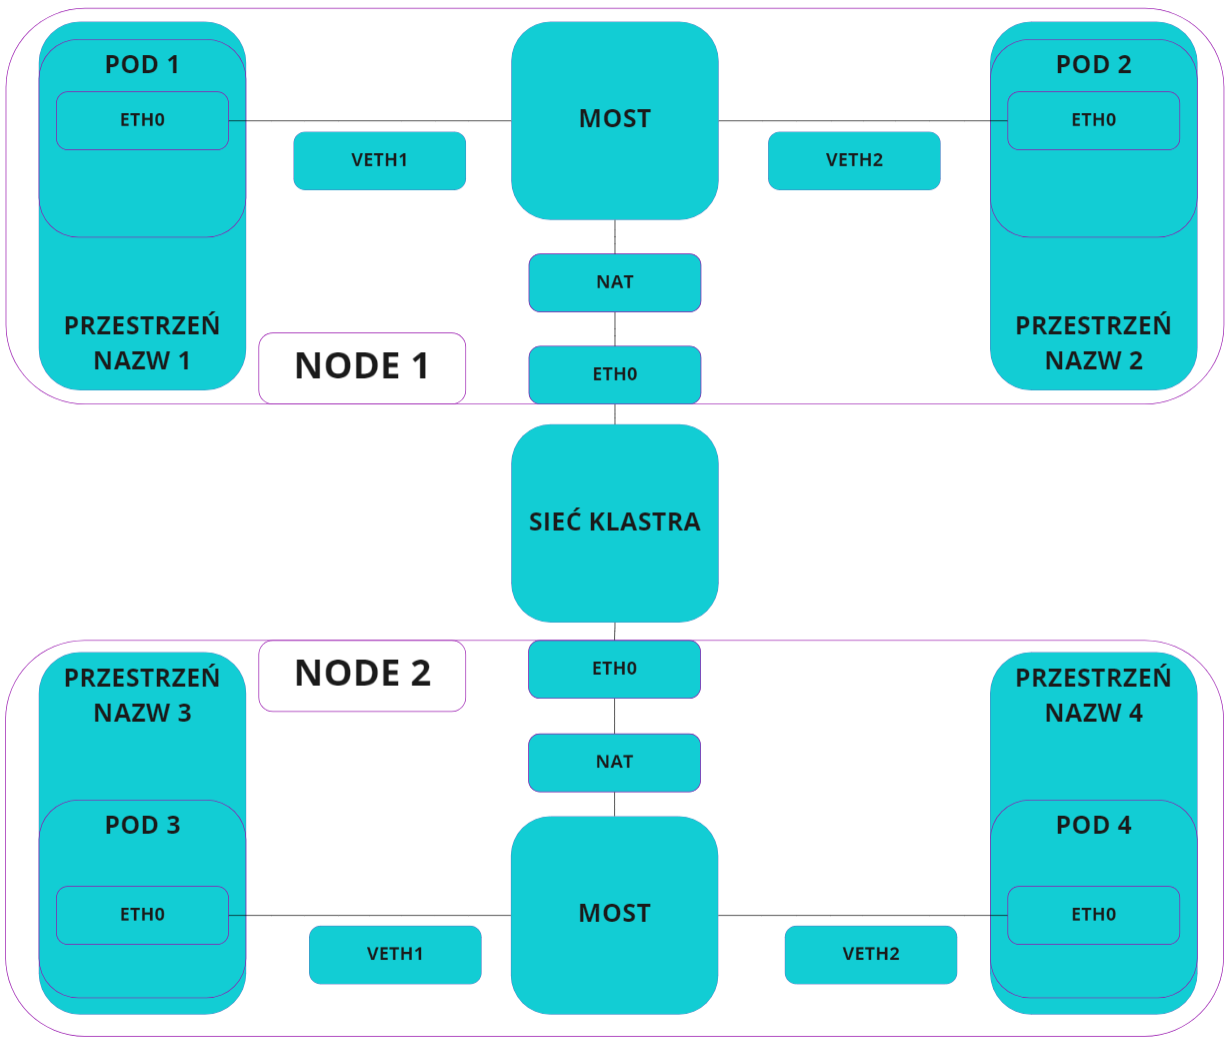
\includegraphics[width=0.9\textwidth]{kubernetes_networking.jpg}
  \caption{Łączność sieciowa w środowisku Kubernetes. Opracowanie własne}
  \label{fig:kubernetes-networking}
\end{figure}
\newpage
\section{Podsumowanie}
\subsection{Możliwości rozszerzenia projektu}

Projekt został przygotowany z myślą o tym, by można było możliwie łatwo tworzyć nowe 
serwisy i integrować je z już istniejącymi. Ważnym elementem ułatwiającym dodawanie 
nowych usług jest jasne zdefiniowane styków oferowanych przez inne serwisy usługowe. 

Na ten moment nie zaimplementowano rozwiązań automatyzujących wykonywanie wymaganych 
czynności w przypadku, gdy warunki rzeczywiste panujące w danym pomieszczeniu nie 
spełniają oczekiwań. Jednym z pomysłów dalszego rozwoju projektu jest wykorzystanie 
towarów produkowanych przez firmę Ikea. Zastosowanie inteligentnego oświetlenia 
wykorzystującego protokół ZigBee pozwoliłoby na automatyczne sterowanie poziomem 
natężenia światła przez aplikację. W tym celu należałoby utworzyć nowy serwis 
wykorzystujący gotową bibliotekę \href{https://github.com/home-assistant-libs/pytradfri}{pytradfri} 
pozwalającą na zarządzanie oświetleniem.

%--------------------------------------------
% Literatura
%--------------------------------------------
\cleardoublepage % Zaczynamy od nieparzystej strony
\printbibliography

%--------------------------------------------
% Spisy (opcjonalne)
%--------------------------------------------
\newpage
\pagestyle{plain}

% Wykaz symboli i skrótów.
% Pamiętaj, żeby posortować symbole alfabetycznie
% we własnym zakresie. Ponieważ mało kto używa takiego wykazu,
% uznałem, że robienie automatycznie sortowanej listy
% na poziomie LaTeXa to za duży overkill.
% Makro \acronymlist generuje właściwy tytuł sekcji,
% w zależności od języka.
% Makro \acronym dodaje skrót/symbol do listy,
% zapewniając podstawowe formatowanie.
% //AB
\vspace{0.8cm}
\acronymlist
\acronym{EiTI}{Wydział Elektroniki i Technik Informacyjnych}
\acronym{PW}{Politechnika Warszawska}
\acronym{ADS}{Addresses Data Service}
\acronym{FDS}{Facilities Data Service}
\acronym{PDS}{Policies Data Service}
\acronym{SDS}{Sensors Data Service}
\acronym{SSHDS}{Sensor State History Data Service}
\acronym{SSDS}{Sensor State Data Service}
\acronym{SSPS}{Sensor State Processing Service}
\acronym{PPS}{Policy Processing Service}
\acronym{EAS}{Employee Application Service}
\acronym{AAS}{Admin Application Service}
\acronym{EA}{Employee Application}
\acronym{AA}{Admin Application}

\listoffigurestoc     % Spis rysunków.
\vspace{1cm}          % vertical space
\listoftablestoc      % Spis tabel.
\vspace{1cm}          % vertical space
\listofappendicestoc  % Spis załączników


% Używając powyższych spisów jako szablonu,
% możesz tu dodać swój własny wykaz bądź listę,
% np. spis algorytmów.

\end{document} % Dobranoc.
